\documentclass[article]{jss}

\newif\ifen
\newif\ifes
\newcommand{\en}[1]{\ifen#1\fi}
\newcommand{\es}[1]{\ifes#1\fi}
\entrue
\usepackage[utf8]{inputenc}

%\newcommand{\jan}{%
%  \en{January}%
%  \es{Enero}
%}

\usepackage{caption}
\usepackage{subcaption}
\usepackage{amsmath} %para escribir funci\'on partida , matrices
\usepackage{amsthm} %para numerar definciones y teoremas
\usepackage{amsfonts} % \mathbb{N} -> conjunto de los n\'umeros naturales

\usepackage{bm} % \bm{\alpha} bold greek symbol
\usepackage[makeroom]{cancel} % \cancel{} \bcancel{} etc
\usepackage{wrapfig} % \begin{wrapfigure} Pone figura al lado del texto
\usepackage{mdframed}
\usepackage{algorithm}
\usepackage{comment}
%\usepackage{quoting}
\usepackage{mathtools}
\usepackage{tikz}
\usepackage{csvsimple}
\usepackage{listings}
\usepackage{hyperref}
\usepackage{todonotes}
\definecolor{dkgreen}{rgb}{0,0.6,0}
\definecolor{mauve}{rgb}{0.58,0,0.82}


% tikzlibrary.code.tex
%
% Copyright 2010-2011 by Laura Dietz
% Copyright 2012 by Jaakko Luttinen
%
% This file may be distributed and/or modified
%
% 1. under the LaTeX Project Public License and/or
% 2. under the GNU General Public License.
%
% See the files LICENSE_LPPL and LICENSE_GPL for more details.

% Load other libraries

%\newcommand{\vast}{\bBigg@{2.5}}
% newcommand{\Vast}{\bBigg@{14.5}}
% \usepackage{helvet}
% \renewcommand{\familydefault}{\sfdefault}

\usetikzlibrary{shapes}
\usetikzlibrary{fit}
\usetikzlibrary{chains}
\usetikzlibrary{arrows}

% Latent node
\tikzstyle{latent} = [circle,fill=white,draw=black,inner sep=1pt,
minimum size=20pt, font=\fontsize{10}{10}\selectfont, node distance=1]
% Observed node
\tikzstyle{obs} = [latent,fill=gray!25]
% Invisible node
\tikzstyle{invisible} = [latent,minimum size=0pt,color=white, opacity=0, node distance=0]
% Constant node
\tikzstyle{const} = [rectangle, inner sep=0pt, node distance=0.1]
%state
\tikzstyle{estado} = [latent,minimum size=8pt,node distance=0.4]
%action
\tikzstyle{accion} =[latent,circle,minimum size=5pt,fill=black,node distance=0.4]
\tikzstyle{fijo} =[latent,circle,minimum size=5pt,fill=black]


% Factor node
\tikzstyle{factor} = [rectangle, fill=black,minimum size=10pt, draw=black, inner
sep=0pt, node distance=1]
% Deterministic node
\tikzstyle{det} = [latent, rectangle]

% Plate node
\tikzstyle{plate} = [draw, rectangle, rounded corners, fit=#1]
% Invisible wrapper node
\tikzstyle{wrap} = [inner sep=0pt, fit=#1]
% Gate
\tikzstyle{gate} = [draw, rectangle, dashed, fit=#1]

% Caption node
\tikzstyle{caption} = [font=\footnotesize, node distance=0] %
\tikzstyle{plate caption} = [caption, node distance=0, inner sep=0pt,
below left=5pt and 0pt of #1.south east] %
\tikzstyle{factor caption} = [caption] %
\tikzstyle{every label} += [caption] %

\tikzset{>={triangle 45}}

%\pgfdeclarelayer{b}
%\pgfdeclarelayer{f}
%\pgfsetlayers{b,main,f}

% \factoredge [options] {inputs} {factors} {outputs}
\newcommand{\factoredge}[4][]{ %
  % Connect all nodes #2 to all nodes #4 via all factors #3.
  \foreach \f in {#3} { %
    \foreach \x in {#2} { %
      \path (\x) edge[-,#1] (\f) ; %
      %\draw[-,#1] (\x) edge[-] (\f) ; %
    } ;
    \foreach \y in {#4} { %
      \path (\f) edge[->,#1] (\y) ; %
      %\draw[->,#1] (\f) -- (\y) ; %
    } ;
  } ;
}

% \edge [options] {inputs} {outputs}
\newcommand{\edge}[3][]{ %
  % Connect all nodes #2 to all nodes #3.
  \foreach \x in {#2} { %
    \foreach \y in {#3} { %
      \path (\x) edge [->,#1] (\y) ;%
      %\draw[->,#1] (\x) -- (\y) ;%
    } ;
  } ;
}

% \factor [options] {name} {caption} {inputs} {outputs}
\newcommand{\factor}[5][]{ %
  % Draw the factor node. Use alias to allow empty names.
  \node[factor, label={[name=#2-caption]#3}, name=#2, #1,
  alias=#2-alias] {} ; %
  % Connect all inputs to outputs via this factor
  \factoredge {#4} {#2-alias} {#5} ; %
}

% \plate [options] {name} {fitlist} {caption}
\newcommand{\plate}[4][]{ %
  \node[wrap=#3] (#2-wrap) {}; %
  \node[plate caption=#2-wrap] (#2-caption) {#4}; %
  \node[plate=(#2-wrap)(#2-caption), #1] (#2) {}; %
}

% \gate [options] {name} {fitlist} {inputs}
\newcommand{\gate}[4][]{ %
  \node[gate=#3, name=#2, #1, alias=#2-alias] {}; %
  \foreach \x in {#4} { %
    \draw [-*,thick] (\x) -- (#2-alias); %
  } ;%
}

% \vgate {name} {fitlist-left} {caption-left} {fitlist-right}
% {caption-right} {inputs}
\newcommand{\vgate}[6]{ %
  % Wrap the left and right parts
  \node[wrap=#2] (#1-left) {}; %
  \node[wrap=#4] (#1-right) {}; %
  % Draw the gate
  \node[gate=(#1-left)(#1-right)] (#1) {}; %
  % Add captions
  \node[caption, below left=of #1.north ] (#1-left-caption)
  {#3}; %
  \node[caption, below right=of #1.north ] (#1-right-caption)
  {#5}; %
  % Draw middle separation
  \draw [-, dashed] (#1.north) -- (#1.south); %
  % Draw inputs
  \foreach \x in {#6} { %
    \draw [-*,thick] (\x) -- (#1); %
  } ;%
}

% \hgate {name} {fitlist-top} {caption-top} {fitlist-bottom}
% {caption-bottom} {inputs}
\newcommand{\hgate}[6]{ %
  % Wrap the left and right parts
  \node[wrap=#2] (#1-top) {}; %
  \node[wrap=#4] (#1-bottom) {}; %
  % Draw the gate
  \node[gate=(#1-top)(#1-bottom)] (#1) {}; %
  % Add captions
  \node[caption, above right=of #1.west ] (#1-top-caption)
  {#3}; %
  \node[caption, below right=of #1.west ] (#1-bottom-caption)
  {#5}; %
  % Draw middle separation
  \draw [-, dashed] (#1.west) -- (#1.east); %
  % Draw inputs
  \foreach \x in {#6} { %
    \draw [-*,thick] (\x) -- (#1); %
  } ;%
}



\newcommand{\vm}[1]{\mathbf{#1}}
\newcommand{\N}{\mathcal{N}}
\newcommand\hfrac[2]{\genfrac{}{}{0pt}{}{#1}{#2}} %\frac{}{} sin la linea del medio

\usepackage{listings}
\lstset{
  language=Python,
  aboveskip=3mm,
  belowskip=3mm,
  showstringspaces=true,
  columns=flexible,
  basicstyle={\small\ttfamily},
  numbers=none,
  numberstyle=\tiny\color{gray},
  keywordstyle=\color{blue},
  commentstyle=\color{dkgreen},
  stringstyle=\color{mauve},
  breaklines=true,
  breakatwhitespace=true,
  tabsize=4
}


%% -- LaTeX packages and custom commands ---------------------------------------

%% recommended packages
\usepackage{thumbpdf,lmodern}

%% another package (only for this demo article)
\usepackage{framed}

%% new custom commands
\newcommand{\class}[1]{`\code{#1}'}
\newcommand{\fct}[1]{\code{#1()}}


%% -- Article metainformation (author, title, ...) -----------------------------

%% - \author{} with primary affiliation
%% - \Plainauthor{} without affiliations
%% - Separate authors by \And or \AND (in \author) or by comma (in \Plainauthor).
%% - \AND starts a new line, \And does not.
\author{Gustavo Landfried \\Universidad de Buenos Aires
   \And Matias Mazzanti \\Universidad de Buenos Aires
   \And Esteban Mocskos \\Universidad de Buenos Aires}
\Plainauthor{Achim Zeileis, Matias Mazzanti, Esteban Mocskos }

%% - \title{} in title case
%% - \Plaintitle{} without LaTeX markup (if any)
%% - \Shorttitle{} with LaTeX markup (if any), used as running title
\title{TrueSkill Through Time: the \proglang{Python} Package}
\Plaintitle{TrueSkill Through Time: the Python Package}
\Shorttitle{TrueSkill Through Time: the \proglang{Python} Package}

%% - \Address{} of at least one author
%% - May contain multiple affiliations for each author
%%   (in extra lines, separated by \emph{and}\\).
%% - May contain multiple authors for the same affiliation
%%   (in the same first line, separated by comma).
\Address{
  Gustavo Andr\'es Landfried\\
  Departamento de Computaci\'on\\
  Facultad de Ciencias Exactas y Naturales\\
  Universidad de Buenos Aires\\
  Buenos Aires, Argentina\\
  E-mail: \texttt{gustavolandfried@gmail.com}\\

  \vspace{0.3cm}

  Matias Mazzanti\\
  Departamento de F\'isica\\
  Facultad de Ciencias Exactas y Naturales\\
  Universidad de Buenos Aires\\
  Buenos Aires, Argentina\\

  \vspace{0.3cm}

  Esteban Mocskos\\
  Departamento de Computaci\'on\\
  Facultad de Ciencias Exactas y Naturales\\
  Universidad de Buenos Aires\\
  Buenos Aires, Argentina\\
  \emph{and}\\
  Departamento de Computaci\'on\\
  Facultad de Ciencias Exactas y Naturales\\
  Universidad de Buenos Aires\\
  Buenos Aires, Argentina\\
}




























%% - \Abstract{} almost as usual
\en{
\Abstract{
 \pkg{ttt} package is a \proglang{Python} implementation of TrueSkill Through Time (TTT), an enhancement of TrueSkill algorithm, widely used by the video game industry for skill estimation.
 TTT is a probabilistic model for general pairwise-comparison.
 A nice feature is the use of a single graphical model for the entire history of events.
 The posterior distribution is computed based on an efficient variationl algorithm, known as expectation propagation.
 As a result, the inference procedure requires only a few linear-time iterations over the data.
 This algorithm outperforms competing estimations in terms of model evidence, and scales to millions of parameters.
 We offer an easy to use interface, compatible with the current \code{trueskill} package for \proglang{Python}.
}
}

\es{
\Abstract{ Traducir
}
}

%% \Keywords{JSS, style guide, comma-separated, not capitalized, \proglang{R}} with LaTeX markup, at least one required
%% - \Plainkeywords{JSS, style guide, comma-separated, not capitalized, R} without LaTeX markup (if necessary)
%% - Should be comma-separated and in sentence case.

\Keywords{TrueSkill, ranking, skill, education, sports, games, Bayesian inference, \proglang{Python}}
\Plainkeywords{TrueSkill, ranking, skill, education, sports, games,  Bayesian inference, Python}

\begin{document}
\lstset{language=Python}

%% -- Introduction -------------------------------------------------------------

%% - But should typically have some discussion of both _software_ and _methods_.
%% - Use \proglang{}, \pkg{}, and \code{} markup throughout the manuscript.
%% - If such markup is in (sub)section titles, a plain text version has to be
%%   added as well.
%% - All software mentioned should be properly \cite-d.
%% - All abbreviations should be introduced.
%% - Unless the expansions of abbreviations are proper names (like "Journal of Statistical Software" above) they should be in sentence case (like "generalized linear models" below).

\section[Introduction: Count data regression in R]{Introduction: } \label{sec:intro}

\todo[inline]{Me gusta que intentas poner un poco de intro, pero no me parece que quede bien empezar con preguntas}
%
\en{What are the skills of the people?}
\es{¿Cu\'ales son las habilidades de las personas?}
%   
\en{How difficult are the challenges they face?}
\es{¿Cu\'an dif\'iciles son los desaf\'ios que enfrentan?}
%
\en{How are their learning curves over time?}
\es{¿C\'omo son sus curvas de aprendizaje en el tiempo?}
%
\en{What is the overall pattern and how variable is it?}
\es{¿Cu\'al es el patr\'on general y cu\'an variable es?}
%
\en{Knowing people's abilities is crucial in the area of education and sports, among others.}
\es{Conocer las habilidades de las personas es crucial en el \'area de la educaci\'on y los deportes, entre otros.}
%
\en{In the context of interventions, it makes it possible to avoid exposing agents to imbalanced challenges.}
\es{En las contexto de intervenciones, permite evitar exponer a los agentes a desaf\'ios desproporcionados.}
%
\en{For research purposes, the ratings can be made available to subjects and the general public, stimulating interest and engagement.}
\es{Con fines de investigaci\'on, las calificaciones pueden ponerse a disposici\'on de los sujetos y del p\'ublico general, estimulando as\'i el inter\'es y la participaci\'on.}
%
\en{However, since it is a complex variable, it is generally impossible to measure it directly (i.e. hidden variable).}
\es{Sin embargo, al ser una variable compleja, generalmente es imposible medirla directamente (aka variable oculta).}
%
\en{In practice, the best we can do is estimate it from its direct observable consequences.}
\es{En la pr\'actica, lo mejor que podemos hacer es estimarla a partir de sus consecuencias observables m\'as directas.}
%
\en{The most widely used sources of information in education and sports are the outcomes of problem solving and competition between opponents, respectively.}
\es{Las fuentes de informaci\'on m\'as utilizadas en educaci\'on y deportes provienen del producto de resoluci\'on de problemas y de competencia entre oponentes, respectivamente.}
%
\en{The naive solution, frequency of positive results, is not a good indicator essentially because it also depends on the difficulty of the challenges.}
\es{La soluci\'on ingenua, frecuencia de resultados positivos, no es un buen indicador fundamentalmente porque depende tambi\'en de la dificultad de los desaf\'ios.}
%
\en{For that reason, all conventional models are underpinned by pairwise comparisons.}
\es{Por esa raz\'on, todos los modelos convencionales se basan en \emph{pairwise comparisons}.}
%
\en{Since the first generative models, proposed almost a century ago by~\cite{thurstone1927-comparativeJugement} and~\cite{zermelo1929-translation}, it is assumed that the probability of an observed result, $r$, depends on the difference in strength, $d$, between the agent and their target.}
\es{Ya los primeros modelos generativos, propuestos hace casi un siglo por~\cite{thurstone1927-comparativeJugement} y~\cite{zermelo1929-translation}, suponen que la probabilidad de un resultado observado, $r$, depende de la diferencia de escala, $d$, entre el agente y su objetivo.}
%
\begin{equation} \label{eq:pairwise-comparision}
p(\,r \,|\, d_{ij}\,) 
\end{equation}
%
\en{The field was revitalized after 20 years by the publications of~\cite{bradley1952-pairedComparisions} and~\cite{mosteller1951-remarks}.}
\es{El campo revitaliz\'o 20 a\~nos despu\'es gracias a las publicaciones de \cite{bradley1952-pairedComparisions} y~\cite{mosteller1951-remarks}.}
%
\en{Nowadays, the most widely used skill estimators are those proposed by~\cite{elo1961-uscf},~\cite{glikman_gliko_2},~\cite{herbrich2006-trueskill}, and some of the Item-Response Theory variants compiled by~\cite{vanDerLinden2016-handbookIRT_1} and~\cite{fox2010-bayesianIRT}.}
\es{Actualmente, los estimadores de habilidades m\'as utilizados son los propuestos por~\cite{elo1961-uscf},~\cite{glikman_gliko_2},~\cite{herbrich2006-trueskill}, y algunas de las variantes de la\emph{Item-Response Theory} recopiladas por~\cite{vanDerLinden2016-handbookIRT_1} y~\cite{fox2010-bayesianIRT}.}
%
\en{Remarkably, they all share the same underlying generative model.}
\es{Notablemente, todos comparten el mismo modelo generativo subyacente.}
%
\en{The main difference in respect to their representations is limited to the choice of one of two very similar cumulative probability distributions to define the equation~\ref{eq:pairwise-comparision}: the logistic function or the cumulative Gaussian one.}
\es{Respecto de su representaci\'on, la principal diferencia se limita a la elecci\'on de una de dos distribuciones de probabilidad acumulativa, muy similares entre s\'i, para definir la ecuaci\'on~\ref{eq:pairwise-comparision}: la funci\'on log\'istica o la Gaussiana acumulativa.}
%
\en{The most substantive differences are methodological differences: alternative methods for solving the shared probabilistic model.}
\es{Las diferencias sustantivas son diferencias metodol\'ogicas: m\'etodos alternativos para resoluci\'on de el modelo probabil\'istico.}

% Cambio de parrafo.

\begin{figure}[h!]
\centering \small
    \tikz{         
    \node[det, fill=black!10] (r) {$r_{ij}$} ; 
    \node[const, left=of r, xshift=-1.35cm] (r_name) {\small \en{Result}\es{Resultado}:}; 
    \node[const, right=of r] (dr) {\normalsize $ r_{ij} = (d_{ij}>0)$}; 

    \node[latent, above=of r, yshift=-0.45cm] (d) {$d_{ij}$} ; %
    \node[const, right=of d] (dd) {\normalsize $ d_{ij}=p_i-p_j$}; 
    \node[const, left=of d, xshift=-1.35cm] (d_name) {\small \en{Difference}\es{Diferencia}:};
    
    \node[latent, above=of d, xshift=-0.8cm, yshift=-0.45cm] (p1) {$p_i$} ; %
    \node[latent, above=of d, xshift=0.8cm, yshift=-0.45cm] (p2) {$p_j$} ; %
    \node[const, left=of p1, xshift=-0.55cm] (p_name) {\small \en{Performance}\es{Rendimiento}:}; 

    \node[accion, above=of p1,yshift=0.3cm] (s1) {} ; %
    \node[const, right=of s1] (ds1) {$s_i$};
    \node[accion, above=of p2,yshift=0.3cm] (s2) {} ; %
    \node[const, right=of s2] (ds2) {$s_j$};
    
    \node[const, right=of p2] (dp2) {\normalsize $p \sim \N(s,\beta^2)$};

    \node[const, left=of s1, xshift=-.85cm] (s_name) {\small \en{Skill}\es{Habilidad}:}; 
    
    \edge {d} {r};
    \edge {p1,p2} {d};
    \edge {s1} {p1};
    \edge {s2} {p2};
    %\node[invisible, right=of p2, xshift=4.35cm] (s-dist) {};
}
     \caption{
     \en{Clasical generative model in which hidden skills cause the observable results through the difference of random performances.}
    \es{Modelo generativo cl\'asico en la que las habilidades ocultas causan los resultados observables a trav\'es de la diferencia de rendimientos aleatorios.}
    %
    \en{The graphical representation defines a joint probability distribution.}
    \es{La representaci\'on gr\'afica define una distribuci\'on de probabilidad conjunta.}
    %
    \en{Black dots denote constant values.}
    \es{Los puntos negros denotan valores constantes.}
    %
    \en{The big circles and squares indicate continuous and discrete random variables respectively.}
    \es{Los c\'irculos y cuadrados indican variables aleatorias continuas y discretas respectivamente.} 
    %
    \en{Observable variables are painted gray and hidden ones are left blank.}
    \es{Las variables observables se pintan de gris y las variable ocultas se dejan en blanco.}
    %
    \en{The arrows represent causal relationships and the functions define them.}
    \es{Las flechas representan relaciones causales y las funciones las definen.}
    }
    \label{fig:generative_model}
\label{modelo}
\end{figure}

% Cambio de parrafo

\en{A breakthrough took place with the methodology developed by~\cite{elo1961-uscf} for the US Chess Federation (USCF), which is still used by the International Chess Federation (FIDE).}
\es{Un gran avance produjo la metodolog\'ia desarrollada por~\cite{elo1961-uscf} para la Federaci\'on de Ajedrez de los Estados Unidos (USCF), adoptada hasta el d\'ia de hoy por la Federaci\'on Internacional De Ajedrez (FIDE).}
%
\en{Figure~\ref{fig:generative_model} provides a graphical representation in which hidden skill generate observable results.}
\es{La figura~\ref{fig:generative_model} ofrece una representaci\'on gr\'afica en la que las habilidades ocultas generan los resultados observables.}
%
\en{The causal relationship is not direct.}
\es{La relaci\'on causal no es directa.}
%
\en{Although agents may have a specific skill at any given time ($s$), the performance ($p$) they exhibit in an event depends on an undetermined number of unknown factors, which are modeled as random noise ($\beta$), $\N(p\,|\,s,\beta^2)$.}
\es{Si bien los agentes pueden tener una habilidad espec\'ifica en cada momento ($s$), el desempe\~no ($p$) que exhiben en cada evento depende de una cantidad indeterminada de factores desconocidos, los que se modelan como ruido aleatorio ($\beta$), $\N(p\,|\,s,\beta^2)$.}
%
\en{According to the model, the observed results are a direct consequence of the difference of those hidden performances, $d_{ij}=p_i - p_j$.}
\es{Según el modelo, los resultados son una consecuencias directa de la diferencia de esos rendimientos ocultos, $d_{ij}=p_i - p_j$.}
%
\en{An agent gets a positive result when he outperforms his opponent, $r_{ij} = (d_{ij} > 0)$.}
\es{Un agente obtiene un resultado positivo cuando supera el rendimiento de su adversario, $r_{ij} = (d_{ij} > 0)$.}
%
\en{By observing a result we can deduce, given the hypotheses, the order of the hidden performances that actually occurred in that event, and its a priori probability.}
\es{Al observar un resultado podemos deducir, dadas las hip\'otesis, el orden de los rendimientos ocultos que en efecto ocurri\'o en ese evento, y su probabilidad a priori.}
%
\en{Elo's methodological solution extremely simple and astute: update the current estimate based on our surprise.}
\es{La soluci\'on metodol\'ogica de Elo es extremadamente sencilla y astuta: actualizar la estimaci\'on actual en funci\'on de nuestra sorpresa.}
%
\begin{equation}
 \Delta = \underbrace{y_{ij}}_{\hfrac{\text{Direction}}{\text{(Sign)}}}\underbrace{\left(1-p(\,r_{ij}\,|\,s_i,s_j\,)\right)}_{\hfrac{\text{Magnitud}}{\text{(Surprise)}}}
\end{equation}
%
\en{Where $y_{ij}$ is $1$ for winners and $-1$ for losers, and the probability of the observed result given the a priori estimates are derived from Figure~\ref{fig:generative_model}.}
\es{Donde $y_{ij}$ es $1$ para ganadores y $-1$ para perdedores y la probabilidad del resultado observado dadas las estimaciones a priori se deriva de la figura~\ref{fig:generative_model}. }
%
\en{Unlikely results would indicate that the current estimates are not entirely correct and should be updated to a greater extent than if they had occurred as expected.}
\es{Los resultados poco probables indicar\'ian que las estimaciones actuales no son del todo correctas y deber\'ian actualizarse en mayor medida que si hubieran ocurrido como se esperaba.}
%
\begin{equation}\label{eq:elo_update}
 s_i^{\text{new}} = s_i^{\text{old}} + \Delta
\end{equation}
%
\en{This solution can recover the relative scale of the agents, starting from arbitrary initial values.}
\es{Esta soluci\'on puede recuperar la escala relativa de los agentes, partiendo de de valores iniciales arbitrarios.}
%
\en{However, it does have some major weaknesses.}
\es{Sin embargo, tiene algunas debilidades importantes.}
%
\en{Because of the lack of a notion of uncertainty about the estimates, what one agent loses in equation~\ref{eq:elo_update} is acquired by the other.}
\es{Debido a la falta de una noci\'on de incertidumbre sobre las estimaciones, lo que un agente pierde en la ecuaci\'on~\ref{eq:elo_update} lo adquiere el otro.}
%
\en{As newly estimates tend to generate high surprise, their presence can abruptly modify estimates that had already converged correctly.}
\es{Como las estimaci\'on nuevas tienden a generan alta sorpresa, su presencia puede modificar bruscamente estimaciones que ya hab\'ian convergido correctamente.}
%
\en{And ad-hoc solution was proposed to breaks the symmetry of equation~\ref{eq:elo_update}: reduce the impact of $\Delta$ based on how many times the agent was already seen by the system.}
\es{Una soluci\'on ad-hoc fue propuesta para romper la simetr\'ia de la ecuaci\'on~\ref{eq:elo_update}: reducir el impacto de $\Delta$ en funci\'on de las veces que el agente ya fue visto por el sistema.}
%
\en{That is the role played by the famous K-factor used by FIDE.}
\es{Ese es rol que desempe\~na el famoso K-factor usado por la FIDE.}
%

% Cambio de parrafo

\en{Probability Theory provides us with a consistent framework for quantifying the uncertainty of our beliefs~\cite{bishop2006-PRML}.}
\es{La Teor\'ia de la Probabilidad nos proporciona un marco consistente para cuantificar la incertidumbre de nuestras creencias~\citep{bishop2006-PRML}.}
%
\en{The use of probability theory to handle uncertainty, known as Bayesian inference, is now widely adopted in the area of artificial intelligence and machine learning primarily because it has proved to be a extremely useful tool in practice.}
\es{El uso de la teor\'ia de la probabilidad para manejar la incertidumbre, conocida como inferencia bayesiana, est\'a hoy adopta de manera generalizada en el \'ambito de la inteligencia artificial y el aprendizaje autom\'atico fundamentalmente porque ha mostrado ser un instrumento sumamente útil en la pr\'actica.}
%
\en{It is not however an ad-hoc choice.}
\es{No es sin embargo una elecci\'on ad-hoc.}
%
\en{Any system that represent degrees of belief by a numerical value, consistent with classical deductive logic and a set of axioms encoding commonsense reasoning, will necessarily be isomorphic to probability theory~\citep{cox1946-reasonableExpectation,vanHorn2003-guideCoxTheorem}.}
\es{Cualquier sistema que represente grados de creencia mediante un valor num\'erico, consistente con la l\'ogica deductiva cl\'asica y un conjunto de axiomas que codifican el razonamiento de sentido común,  ser\'a necesariamente isom\'orfico a la teor\'ia de la probabilidad~\citep{cox1946-reasonableExpectation,vanHorn2003-guideCoxTheorem}.}
%
\en{And all of the probabilistic inference, no matter how complex, can be solved in terms of two simple equations: the~\ref{eq:sum_rule} and the~\ref{eq:product_rule}.}
\es{Y toda inferencia probabil\'istica, no importa cuan compleja ella sea, puede ser resuelta a trav\'es de dos simples ecuaciones: la~\ref{eq:sum_rule} y la~\ref{eq:product_rule}.}
%
\begin{equation} \label{eq:sum_rule}
 \tag{\en{sum rule}\es{regla de la suma}}
 p(x) = \sum_{y \in Y} p(x,y)
\end{equation}
%
\en{This means that any marginal distribution, $p(x)$, can be obtained by integrating the joint distribution $p(x,y)$, in this case by summing out all of the $Y$ values.}
\es{Esto significa que cualquier distribuci\'on marginal $p(x)$ puede ser obtenida integrando la distribuci\'on conjunta $p(x,y)$, en este caso sumando todos los valores de $Y$.}
%
\begin{equation}\label{eq:product_rule}
\tag{\en{product rule}\es{regla del producto}}
 p(x,y) = p(x|y) p(y)
\end{equation}
%
\en{Additionally, any joint distribution can be expressed as the product of one-dimensional conditional distributions.}
\es{Adem\'as, cualquier distribuci\'on conjunta puede ser expresada como el producto de distribuciones condicionales uni-dimensionles.}
%
\en{This rule, together with the symmetry property $p(x,y) = p(y,x)$, we can immediately obtain the~\ref{eq:bayes_theorem},}
\es{Esta regla, junto con la propiedad de simetr\'ia $p(x,y) = p(y,x)$, podemos obtenemos inmediatamente el~\ref{eq:bayes_theorem},}
%
\begin{equation}\label{eq:bayes_theorem}
\tag{\en{Bayes' theorem}\es{Teorema de bayes}}
 p(y|x) = \frac{p(x|y)p(y)}{p(x)}
\end{equation}
%
\en{The inferential use of Bayes' theorem plays a central role in modern statistical learning techniques.}
\es{El uso inferencial del teorema de bayes juega un rol central en las t\'ecnicas modernas de aprendizaje estad\'isitico.}
%
\en{This formula allows us to optimally update our beliefs about a set of hypotheses, given a model and the data.}
\es{Esta expresi\'on nos permite actualizar de forma \'optima nuestras creencia sobre ciertas hip\'otesis, dado un modelo y los datos.}
%
\begin{equation}\label{eq:inference}
 \underbrace{p(\text{\en{Hypotesis}\es{Hip\'otesis}}|\text{\en{Data}\es{Datos}})}_{\text{Posterior\es{i}}} = \frac{\overbrace{p(\text{\en{Data}\es{Datos}}|\text{\en{Hypotesis}\es{Hip\'otesis}})}^{\text{\en{Likelihood}\es{Verosimilitud}}}\overbrace{p(\text{\en{Hypotesis}\es{Hip\'otesis}})}^{\text{Prior\es{i}}}}{\underbrace{p(\text{\en{Data}\es{Datos}})}_{\text{Evidenc\en{e}\es{ia}}}}
\end{equation}
%
\en{where the role played by the model is left implicit.}
\es{donde el lugar que ocupa el modelo queda impl\'icito.}
%

% Nuevo P\'arrafo

\en{In our case, the hypotheses are the people's ability, the data is given by the observed results, and the model is defined by the figure~\ref{fig:generative_model}.}
\es{En nuestro caso, las hip\'otesis son las habilidades de las personas, los datos son los resultados y el modelo est\'a definido por la figure~\ref{fig:generative_model}.}
%
\en{With a probability distribution that represents our prior beliefs about people's abilities, we can obtain the exact posterior belief distribution by the use of the sum and product rules.}
\es{Con una distribuci\'on de probabilidad que represente nuestras creencias a priori sobre las habilidad de las personas, podemos obtener la distribuci\'on de creencias a posterori exacta usando tan solo las reglas de la suma y el producto.}
%
\en{}
\es{En el caso ganador}
%
\begin{figure}[t!]
\centering
\en{\includegraphics[page={1},width=.6\linewidth]{figures/posterior_win}}
\es{\includegraphics[page={2},width=.6\linewidth]{figures/posterior_win}}
\caption{
\en{Exact belief update for the winning case.}
\es{Actualizaci\'on de creencias exacta para el caso ganador.}
%
\en{The prior is a Gaussian distribution.}
\es{La distribuci\'on a priori es una Gaussiana.}
%
\en{The likelihood is a cumulative Gaussian distribution.}
\es{La verosimilitud es la acumulada de una distribuci\'on Gaussiana.}
%
\en{The posterior distribution is obtained as the product of the prior and the likelihood.}
\es{La distribuci\'on a posteriori se obtiene como el producto de la distribuci\'on a priori y la verosimilitud.}
%
\en{Note that the distributions are not on the same scale: the prior integrates 1, while the likelihood goes from 0 to 1.}
\es{Notar que las distribuciones no est\'an en la misma escala: la distribuci\'on a priori integra 1, mientras que la verosimilitud va de 0 a 1.}
%
\en{It is interesting to note that likelihood works as a filter for prior beliefs.}
\es{Es interesante observar que la verosimilitud funciona como filtro de las creencias a priori.}
%
\en{In regions of very high skill, where an observed winning result would not generate any surprises, the a posteriori distribution stays next to the prior.}
\es{En las regiones de habilidad muy alta, donde un resultado ganador observado no generar\'ia ninguna sorpresa, la distribuci\'on a posteriori se queda junto al prior.}
%
\en{In regions of very low skill, where an observed winning result would be very surprising, the subsequent one loses almost all its density.}
\es{En las regiones de habilidad muy bajas, donde un resultado observado ganador ser\'ia muy sorprendente, la distribuci\'on a posteriori pierde casi toda su densidad.}
%
\en{It is important to stress that the posterior, although similar, is not a Gaussian.}
\es{Es importante remarcar que la posterior, aunque se parece, no es una Gaussiana.}
}
\label{fig:posterior_win}
\end{figure}
%
\begin{equation} \label{eq:posterior_win}
\underbrace{p(s_i|r_{ij},s_j)}_{\text{Posterior\es{i}}} \propto \underbrace{\Phi(0 \, | s_i - \mu_j , \, 2\beta^2 + \sigma_j^2)}_{\text{\en{Likelihood}\es{Verosimilitud}}} \,  \underbrace{\N(s_i \, | \, \mu_i,\, \sigma_i^2)}_{\text{Prior\es{i}}} 
\end{equation}
%
\en{Where $\Phi$ represents the cumulative Gaussian distribution.}
\es{Donde $\Phi$ representa la distribuci\'on Gaussiana acumulada.}
%
%\en{Figure~\ref{fig:posterior_win} shows, in graphical terms, the updating procedure performed in equation~\ref{eq:posterior_win}.}
%\es{La figura~\ref{fig:posterior_win} muestra, en términos gr\'aficos, el procedimiento de actualizaci\'on que se realiza en la ecuaci\'on~\ref{eq:posterior_win}.}
% 
\en{The posterior distribution is obtained as the product of the prior and the likelihood.}
\es{La distribuci\'on a posteriori se obtiene como el producto de la distribuci\'on a priori y la verosimilitud.}
%
\en{It is interesting to note that likelihood works as a filter for prior beliefs (Figure~\ref{fig:posterior_win}).}
\es{Es interesante observar que la verosimilitud funciona como filtro de las creencias a priori (figura~\ref{fig:posterior_win}).}
%
\en{It is important to stress that the posterior, although similar, is not a Gaussian.}
\es{Es importante remarcar que la posterior, aunque se parece, no es una Gaussiana.}


% Parrafo nuevo

\en{Obtaining the Gaussian that best approximates it would allow us to extend the inference iteratively in time through the use of the posteriors as priors of the following observations.}
\es{Conseguir la Gaussiana que mejor la aproxima nos permitir\'ia extender la inferencia iterativamente en el tiempo a tavés del uso de las posteriors como priors de las siguientes observaciones.}
%
\en{One of the main contributions of~\cite{herbrich2006-trueskill} was to offer an efficient method to find that Gaussian.}
\es{Uno de los principales aportes de~\cite{herbrich2006-trueskill} fue ofrecer un método eficiente para calcular esa Gaussiana.}

% 
% 
% \cite{dangauthier2008-trueskillThroughTime}
% 
% \cite{coulom2008-wholeHistoryRating}
% 
% \cite{maystre2019-pairwise}
% 
% 
% 
% 
% TrueSkill Through Time (TTT) optar por la distribuci\'on normal y ofrece una soluci\'on \'optima.

















%% -- Manuscript ---------------------------------------------------------------

%% - In principle "as usual" again.
%% - When using equations (e.g., {equation}, {eqnarray}, {align}, etc.
%%   avoid empty lines before and after the equation (which would signal a new
%%   paragraph.
%% - When describing longer chunks of code that are _not_ meant for execution
%%   (e.g., a function synopsis or list of arguments), the environment {Code}
%%   is recommended. Alternatively, a plain {verbatim} can also be used.
%%   (For executed code see the next section.)

\section{Models and software} \label{sec:computoAnilitico}


%
\en{It can be shown [SE DEMOSTRARA EN LA SECCIÓN SIGUIENTE], based on Gaussians properties, that the difference of performance $d_{ij}$ is also normally distributed, centered at the skill difference point with double variance.}
\es{}
%
\begin{equation}
 p( \, d_{ij} \,|\,  s_i, s_j\, ) = \N(\, d_{ij} \,|\, s_i - s_j \, , \, 2\beta^2 \,)
\end{equation}
%
\en{This reduces the problem of computing the probability of the game outcome to a single-dimension problem related to the performance difference.}
\es{This reduces the problem of computing the probability of the game outcome to a single-dimension problem related to the performance difference.}
%
\en{Let the result of a game $r_{ij} = \mathbb{I}(d_{ij}>0)$.
The probability of winning, $r_{ij} = 1$, can be computed as:}
\es{}
%
\begin{equation}
p(\,r_{ij}=1\,|\,d_{ij}\,) = p(\,d_{ij} > 0 \,|\, s_i, s_j\,) = \Phi \left(\frac{s_i - s_j}{\sqrt{2}\beta} \right)
\end{equation}
%
where $\Phi$ is the cumulative distribution function of the standard normal distribution, $\N(0, 1)$.




% \begin{figure}[ht!]
% \centering
% \includegraphics[width=.49\linewidth]{Imagenes/Fig6}
% \caption{\small Joint probability of the performance of two players $i$, $j$ under the assumption of $s_i> s_j$ and independence. All lines parallel to the diagonal $ p_i = p_j $ represent ``difference of performances'' isobars $d_{ij} = p_i - p_j$.}
% \label{probaOfWin_2D}
% \end{figure}

% \begin{figure}[ht!]
% \centering
% \includegraphics[width=.49\linewidth]{Imagenes/Fig7}
% \caption{\small The probability of the outcome of a game under the assumptions of the Elo rating system with $s_i> s_j$. The area under the curve in the positive interval ($d_{ij}>0$) is the winning probability for the player $i$, and the area under the curve in the negative interval is the winning probability of player $j$.}
% \label{probaOfWin}
% \end{figure}





--------------------


Para calcular la posterior utilizamos un algoritmo gen\'erico de pasaje de mensajes para \emph{factor graphs} llamado \emph{sum-product algorithm}~\cite{kschischang2001-factorGraphsAndTheSumProductAlgorithm}.
Permite resolver funciones marginales eficientemente mediante el uso de la forma en la cual la funci\'on global se factoriza en el producto de funciones locales simples, cada una dependiente de una subconjunto de variables.

\subsection{Sum-product algorithm}

Un \emph{factor graph} es una grafo bipartito, (relaciones entre nodos variable $v$ y nodos factor $f$).
Los ejes del factor graph representan la relaci\'on matem\'atica ``nodo $v$ es argumento de nodo $f$''.
La estructura del grafo codifica la factorizaci\'on de la funci\'on global.
Pero adem\'as, cuando un grafo de factorizaci\'on (\emph{factor graph}) no contiene ciclos, el grafo codifica tambi\'en las expresiones aritm\'eticas mediante las cuales se puede computar las marginales asociadas a la funci\'on global.

\paragraph{The Sum-Product Update Rule} El mensaje enviado desde un v\'ertice $v$ a trav\'es de un eje $e$ es el producto de la funci\'on local de $v$ (funci\'on indicadora si $v$ es un nodo variable) con todos los mensajes recibidos en $v$ a trav\'es de ejes \emph{distintos} de $e$, integrados para la variable asociada con $e$.

\vspace{0.3cm}

Sea $m_{x \rightarrow f}(x)$ el mensaje enviado por el nodo variable $x$ al nodo factor $f$, y $m_{f \rightarrow x}(x)$ el mensaje enviado por un nodo factor $f$ a un nodo variable $x$.
Sea $n(v)$ el conjunto de nodos vecinos al nodo $v$.
Luego, los mensajes pueden ser expresados del siguiente modo.
\begin{equation}\label{eq:m_v_f} 
m_{x \rightarrow f}(x) = \prod_{h \in n(x) \setminus \{f\} } m_{h \rightarrow x}(x)
\end{equation}
\begin{equation}\label{eq:m_f_v}  
m_{f \rightarrow x}(x) = \int \cdots \int \Big( f(\bm{x}) \prod_{h \in n(f) \setminus \{x\} } m_{h \rightarrow f}(h) \Big) \,  d\bm{x}_{\setminus x}
\end{equation}

donde $\bm{x} = \text{arg}(f)$ es el conjunto de argumentos de la funci\'on $f$. 
Luego, para calcular una marginal cualquiera,
\begin{equation}\label{eq:marginal}
g_i(x_i) = \prod_{h \in n(x_i)} m_{h \rightarrow x_i}
\end{equation}



En el caso de \texttt{TrueSkill},
la funci\'on representada por el factor graph es la distribuci\'on
conjunta $p(\bm{s},\bm{p},\bm{t}|\bm{o},A)$ (Fig.
\ref{factorGraph_trueskill}).

\begin{figure}[t!]
  \centering
  \scalebox{.9}{
  \tikz{ %


        \node[factor] (fr) {} ;
        \node[const, above=of fr] (nfr) {$f_r$}; %
	\node[const, above=of nfr] (dfr) {\large $\mathbb{I}(g\,d_{ab}>0)$}; %
        \node[latent, left=of fr] (d) {$d_j$} ; %
        \node[factor, left=of d] (fd) {} ;
        \node[const, above=of fd] (nfd) {$f_d$}; %
        \node[const, above=of nfd] (dfd) {\large $\mathbb{I}(d_{ab}=t_a - t_b)$}; %
        \node[const, below=of d,yshift=-0.15cm] (j) {\footnotesize con signo $g:=1 - 2*\mathbb{I}(o_a < o_b) $};

        \node[latent, left=of fd,xshift=-0.9cm] (t) {$t_e$} ; %
        \node[factor, left=of t] (ft) {} ;
        \node[const, above=of ft] (nft) {$f_t$}; %
        \node[const, above=of nft,xshift=0.5cm] (dft) {\large $\mathbb{I}(t_e = \sum_{i \in A_e} p_i)$}; %

        \node[latent, left=of ft] (p) {$p_i$} ; %
        \node[factor, left=of p] (fp) {} ;
        \node[const, above=of fp] (nfp) {$f_p$}; %
        \node[const, above=of nfp] (dfp) {\large $N(p_i;s_i,\beta^2)$}; %

        \node[latent, left=of fp] (s) {$s_i$} ; %
        \node[factor, left=of s] (fs) {} ;
        \node[const, above=of fs] (nfs) {$f_s$}; %
        \node[const, above=of nfs] (dfs) {\large $N(s_i;\mu_i,\sigma^2)$}; %

        \edge[-] {d} {fr};
	\edge[-] {fd} {d};
        \edge[-] {fd} {t};
        \edge[-] {t} {ft};
        \edge[-] {ft} {p};
        \edge[-] {p} {fp};
        \edge[-] {fp} {s};
        \edge[-] {s} {fs};

        \plate {personas} {(p)(s)(fs)(nfs)(dfp)(dfs)} {$i \in A_e$}; %
        \node[invisible, below=of ft, yshift=-0.6cm] (inv_below_e) {};
	\node[invisible, above=of ft, yshift=1.1cm] (inv_above_e) {};
	\plate {equipos} {(personas) (t)(ft)(dft) (inv_above_e) (inv_below_e)} {$  \text{con $A$ partici\'on de jugadores }$  \hspace{3cm} $0 < e \leq |A|$}; %
	\node[invisible, below=of fr, yshift=-0.6cm] (inv_below) {};
	\node[invisible, above=of fr, yshift=1.1cm] (inv_above) {};
	\plate {comparaciones} {(fd) (dfd) (d) (fr) (dfr) (inv_below) (inv_above)} {$a$ equipo focal \hspace{0.6cm} $0 < b \leq |A| \ , \ a \neq b$};
        }  }
  \caption{\small Grafo bipartito de la factorizaci\'on (\emph{factor graph}) del modelo \texttt{Trueskill}}
  \label{factorGraph_trueskill}
\end{figure}

\subsection{Solucion exacta}


%\section{Prior predictive y evidencia}

La evidencia es otro nombre para el Prior predictive.
%
\begin{equation*}
\underbrace{P(\text{Belief}|\text{Data})}_{\text{\scriptsize Posterior}} = \frac{\overbrace{P(\text{Data}|\text{Belief})}^{\text{\scriptsize Likelihood}} \overbrace{P(\text{Belief})}^{\text{\scriptsize Prior}} }{\underbrace{P(\text{Data})}_{\hfrac{\hfrac{\text{\scriptsize Evidence or}}{\text{\scriptsize Average likelihood}}}{\text{\scriptsize Prior Predictive}} } }
\end{equation*}




\subsection{Draw}

If draws are permitted, the winning outcome $r_{(j)} < r_{(j+1)}$, requires $t_{r_{(j)}} > t_{r_{(j+1)}} + \epsilon$, and the draw outcome $r_{(j)}=r_{(j+1)}$ requires $|t_{r_{(j)}} > t_{r_{(j+1)}}| \leq \epsilon$ where $\epsilon$ is a draw margin.

\vspace{0.3cm}

The draw margin can be seted by the a given ``empirical draw probability''.
Para entender de donde obtener este valor, debemos recordar que la diferencia de rendimientos verdadera se generan a partir de una distribuci\'on normal centrada en las verdaderas habilidad y con la suma de los desvios asociacios a los rendimientos $\N( \sum_i s_i^{\text{true}} - \sum_j s_j^{\text{true}},(n_1+n_2)\beta^2)$.
Notar que esta distribuci\'on no depende de nuestras creencias, por eso no depende de nuestra incertidumbre $\sigma$. 

\begin{figure}[H]
\centering
  \includegraphics[width=0.5\textwidth]{figures/draw.pdf}
  \caption{La distirbuci\'on verdadera de diferencia entre equipos, $\N( \sum_i s_i^{\text{true}} - \sum_j s_j^{\text{true}},(n_1+n_2)\beta^2)$.}
  \label{fig:draw}
\end{figure}

Intuitivamente sabemos que la probabilidad de empate depende de la diferencia de habilidad.
Por eso, cuando hablamos de \textbf{una} probabilidad emp\'irica, en el fondo estamos pensando \textbf{la} probabilidad emp\'irica para una diferencia de habilidad determinada.
En particular \textbf{la probabilidad de empates para jugadores \emph{si tuviera misma habilidad}}.
En este punto nos estamos mordiendo la cola, porque estamos construyendo el modelo para estimar habilidades justamente porque no las conocemos.
En este punto es bueno remarcar que la probabilidad de empate para jugadores de misma habilidad, así como el $\beta$, es un valor en buen medida arbitraro de nuestro modelo.
Si lo quisieramos estimar, deberíamos proponer una distirbuci\'on de creencias a priori, y actualizarla con nuestro modelo.

\vspace{0.3cm}

Suponiendo que tenemos la probabilidad de empate para oponentes de misma habilidad, para mantener estable el \'area ante diferentes escenarios, el $\epsilon$ debe poder adaptarse.
El \'unico par\'ametro libre en este caso es la cantidad de jugadores en los equipos, que modifica el ancho de la distribuci\'on de la diferencia de habilidad.

\begin{figure}[H]
\centering
  \includegraphics[page=2,width=0.5\textwidth]{figures/draw.pdf}
  \caption{Distribuci\'on de probabilidades de diferencias de rendimientos, y área correspondiente a la probabilidad de empate $0.25$}
  \label{fig:draw}
\end{figure}

Por eso, el $\epsilon$ se dice que depende de, 

\begin{equation}
 \text{Draw probability} = \Phi(\frac{\epsilon}{\sqrt{n_1+n_2}\beta}) - \Phi(\frac{-\epsilon}{\sqrt{n_1+n_2}\beta})
\end{equation}

Donde el denominador se corresponde con el desvio total de los $n_1 + n_2$ jugadores.
Recordar que $\Phi$ es la acumulada de la distribuc\'on Normal estandarizada, centrada en 0. 


 
 
 
 
 
 










\section{Full TrueSkill}

\begin{center}
\tikz{ %        
        \node[factor, xshift=-5cm] (fta) {} ;
        \node[const, right=of fta] (nfta) {$f_{t_0}$}; %
        \node[latent, below=of fta,yshift=-0.5cm] (ta) {$t_0$} ; %
        
        \node[factor] (ftb) {} ;
        \node[const, right=of ftb] (nftb) {$f_{t_1}$}; %
        \node[latent, below=of ftb,yshift=-0.5cm] (tb) {$t_1$} ; %
        
        \node[factor, xshift=5cm] (ftc) {} ;
        \node[const, right=of ftc] (nftc) {$f_{t_2}$}; %        
        \node[latent, below=of ftc,yshift=-0.5cm] (tc) {$t_2$} ; %
        
        \node[factor, below=of tb, xshift=-3cm] (fd1) {} ;
        \node[const, left=of fd1] (nfd1) {$f_{d_0}$}; %        
        \node[latent, below=of fd1,yshift=-1cm] (d1) {$d_{0}$} ; %
        \node[factor, below=of d1,yshift=-1cm] (fr1) {} ;
        
        \node[factor, below=of tb, xshift=3cm] (fd2) {} ;
        \node[const, above=of fd2] (nfd2) {$f_{d_{1}}$}; %        
        \node[latent, below=of fd2,yshift=-1cm] (d2) {$d_{1}$} ; %
        \node[factor, below=of d2,yshift=-1cm] (fr2) {} ;
        
        \edge[-] {ta} {fta,fd1}
        \edge[-] {tb} {ftb,fd1,fd2}
        \edge[-] {tc} {ftc,fd2}
        \edge[-] {d1} {fd1,fr1}
        \edge[-] {d2} {fd2,fr2}
        
        \path[draw, -latex, fill=black!50,sloped] (fd1) edge[bend left,draw=black!50] node[midway,above,color=black!75] {\scriptsize  \emph{loseLikelihood}$(t_1)$} (tb);
        
        \path[draw, -latex, fill=black!50,sloped] (tb) edge[bend left,draw=black!50] node[midway,below,color=black!75] {\scriptsize  \emph{losePosterior}$(t_1)$} (fd1);
        
        \path[draw, -latex, fill=black!50,sloped] (fd2) edge[bend right,draw=black!50] node[midway,above,color=black!75] {\scriptsize \emph{winLikelihood}$(t_1)$} (tb);
        
        \path[draw, -latex, fill=black!50,sloped] (tb) edge[bend right,draw=black!50] node[midway,below,color=black!75] {\scriptsize \emph{winPosterior}$(t_1)$} (fd2);
        
        \path[draw, -latex, fill=black!50,sloped] (fta) edge[bend left,draw=black!50] node[midway,above,color=black!75] {\scriptsize \emph{prior}$(t_0)$} (ta);
        
        \path[draw, -latex, fill=black!50,sloped] (fr1) edge[bend left,draw=black!50] node[midway,above,color=black!75, rotate=180] {\scriptsize \emph{likelihood}$(d_{0})$} (d1);
        
        \path[draw, -latex, fill=black!50,sloped] (d1) edge[bend right,draw=black!50] node[midway,above,color=black!75] {\scriptsize \emph{\ \ posterior}$(d_{0})$} (fd1);
        
        \path[draw, -latex, fill=black!50,sloped] (fd1) edge[bend right,draw=black!50] node[midway,above,color=black!75] {\scriptsize \emph{prior}$(d_{0})$} (d1);
        
        \path[draw, -latex, fill=black!50,sloped] (tc) edge[bend left,draw=black!50] node[midway,above,color=black!75] {\scriptsize \emph{posterior}$(t_0)$} (ftc);
        
        
        %\path[draw, -latex, fill=black!50,sloped] (fr2) edge[bend left,draw=black!50] node[midway,above,color=black!75, rotate=180] {\scriptsize \textbf{5:} \emph{likelihood}$(d_{0})$} (d2);
        
        %\path[draw, -latex, fill=black!50,sloped] (fd2) edge[bend left,draw=black!50] node[midway,above,color=black!75] {\scriptsize \textbf{4:} \emph{prior}$(d_{0})$} (d2);
        
        
} 
\end{center}

\begin{equation}
 p(t_e) = \emph{prior}(t_e) \cdot \emph{looseLikelihood}(t_e) \cdot \emph{winLikelihood}(t_e)
\end{equation}

\begin{equation}
 p(d_i) = \emph{prior}(d_i) \cdot \emph{likelihood}(d_i)
\end{equation}

There is a mutual dependency between the team performance (difference) marginals, $p(d_i)$.
That makes impossible to perform a one shot inference.
The basic idea is to update repeatedly forward and backward all messages in the shortest path between any two marginals $p(d_i)$ until convergence.
The messages that are not yet defined, for example the \emph{winLikelihood}$(t_1)$ in the first forward pass, must be replace it by a neutral form, like a unit scalar or a Gaussian distribution with infinite variance.
If the messages have already been defined, then use the last available definition.

\paragraph{$\bm{\emph{winPosterior}(t_i)}$:}

\begin{equation}
 \begin{split}
  \emph{winPosterior}(t_{i}) = \emph{prior}(t_i) \cdot \emph{winLikelihood}(t_i)
 \end{split}
\end{equation}


\paragraph{$\bm{\emph{losePosterior}(t_i)}$:}

\begin{equation}
 \begin{split}
  \emph{losePosterior}(t_{i}) = \emph{prior}(t_i) \cdot \emph{loseLikelihood}(t_i)
 \end{split}
\end{equation}


\paragraph{$\bm{\emph{prior}(d_i)}$:}

\begin{equation}
 \begin{split}
  \emph{prior}(d_{i}) = \iint \mathbb{I}(d_{i} = t_i - t_{i+1} ) \cdot winPosterior(t_i) \cdot losePosterior(t_{i+1}) \, dt_idt_{i+1} 
 \end{split}
\end{equation}


\paragraph{$\bm{\widehat{\emph{likelihood}}(d_i)}$:}

\begin{equation}
\widehat{p}(d_i) = \emph{prior}(d_i) \, \widehat{\emph{likelihood}}(d_i)
\end{equation}

Following the expectation propagation algorithm, we approximate the \emph{likelihood}$(d_i)$ by approximating the marginal $p(d_i)$ via moment matching, resulting in $\widehat{p}(d_i)$ a Gaussian with the same mean and variance as $p(d_i)$.
\begin{equation}
\begin{split}
 \widehat{p}(d_i) & = \emph{approx}(p(d_i)) = \emph{approx}(\emph{prior}(d_i) \cdot \emph{likelihood}(d_i)) 
 \end{split}
\end{equation}

Then, 
\begin{equation}
\begin{split}
\widehat{\emph{likelihood}}(d_i) &= \frac{\emph{approx}(\emph{prior}(d_i) \cdot \emph{likelihood}(d_i))}{ \emph{prior}(d_i)}
\end{split}
\end{equation}

\paragraph{$\bm{\widehat{\emph{posterior}}(d_i)}$:}


\begin{equation}
\begin{split}
\widehat{\emph{posterior}}(d_i) &= \widehat{\emph{likelihood}}(d_i)
\end{split}
\end{equation}

\paragraph{\emph{loseLikelihood}$\bm(t_{i+1})$:}

\begin{equation}
 \begin{split}
  \emph{loseLikelihood}(t_{i+1}) = \iint \mathbb{I}(d_{i} = t_i - t_{i+1} ) \emph{winPosterior}(t_i) \widehat{\emph{posterior}}(d_i) \, dd_idt_{i+1} 
 \end{split}
\end{equation}


\paragraph{\emph{winLikelihood}$\bm(t_{i})$:}

\begin{equation}
 \begin{split}
  \emph{winLikelihood}(t_{i}) = \iint \mathbb{I}(d_{i} = t_i - t_{i+1} ) \emph{losePosterior}(t_{i+1}) \widehat{\emph{posterior}}(d_i) \, dd_idt_{i+1} 
 \end{split}
\end{equation}





\subsection{TrueSkill through Time (TTT)}

%\todo[inline]{Poner un primer parrafo que le de algo de hilo a la historia}

Consider a game in which $N$ players $\{1, \dots, N\}$ are compete over a period of $T$ time steps or temporal batch (e.g. day, week, month, year).
Denote the series of games outcomes between two players $i$ and $j$ within a temporal batch $t$ by $\vm{y}^t_{ij}(k)$, where $k \in \{1,\dots,K^t_{ij}\}$, with $K^t_{ij}$ the number of games outcomes available for that pair of players in that temporal batch.

\en{
\begin{itemize}
 \item Inference within a temporal batch (day, week, month) depends on the random order chosen for the update. However the results should be independent of the order of games within the temporal batch.
 \item Information across temporal batch is only propagated forward in time, so we can not propagate information backwards.
\end{itemize}
}
\es{\begin{itemize}
		\item Inferencia entre un bache temporal (d\'ia, semana, mes) depende del orden aleatorio elegido para la actualizaci\'on. De todas formas el resultado deberia ser independiente del orden de los juegos dentro de un bache temporal.
		\item La informaci\'on a trav\'es de un bache es solo propagado de manera temporal hacia adelante, no pudiendo propagarla en sentido contrario.
\end{itemize}}


The neighbor factor graph of a temporal skill variable $s_i^t$, is

\begin{center}
\tikz{ %
        \node[latent] (s0) {$s_i^{t-1}$} ; %

        \node[factor, right=of s0,xshift=1cm ] (fs1) {} ;
        \node[const, above=of fs1] (nfs1) {$f_{s_i^{t}}$}; %

        \node[latent, right=of fs1, xshift=1.25cm] (s1) {$s_i^t$} ; %

        \node[factor, right=of s1, xshift=1.25cm ] (fs2) {} ;
        \node[const, above=of fs2] (nfs2) {$f_{s_i^{t+1}}$}; %

        \node[latent, right=of fs2,xshift=1cm] (s2) {$s_i^{t+1}$} ; %

        \node[factor, below=of s1,xshift=-1.4cm,yshift=-1cm] (fp0) {} ;
        \node[const, right=of fp0] (nfp0) {$f_{p_i^{t}(1)}$}; %

        \node[factor, color=white, below=of s1] (fp1) {} ;
        %\node[const, right=of fp1] (nfp1) {$f_{p_i^{t}(2)}$}; %

        \node[factor, below=of s1,xshift=1.4cm,yshift=-1cm] (fp2) {} ;
        \node[const, left=of fp2] (nfp2) {$f_{p_i^{t}(k)}$}; %

        \node[latent, below=of fp0] (p0) {\footnotesize$p_i^{t}(1)$} ; %
        %\node[latent, below=of fp1] (p1) {\footnotesize$p_i^{t}(2)$} ; %
        \node[latent, below=of fp2] (p2) {\footnotesize$p_i^{t}(k)$} ; %

        %\draw[bend right=90] (fs1) arc (s1) node[midway,above]{label};
        %\draw[bend left,->]  (fs1) to node [auto] {Link} (s1);
        \edge[-] {s1} {fp0,fp1,fp2};
        \edge[-] {fp0} {p0};
        %\edge[-] {fp1} {p1};
        \edge[-] {fp2} {p2};
        \edge[-] {fs1} {s0,s1};
        \edge[-] {fs2} {s1,s2};
        %\edge[bend right] {s0} {fs1};
        \path[draw, -latex, fill=black!50] (s0) edge[bend right,draw=black!50] node[midway,below,color=black!75] {\scriptsize \emph{posterior}$(t-1)$} (fs1);
        \path[draw, -latex, fill=black!50] (fs1) edge[bend left,draw=black!50] node[midway,above,color=black!75] {\scriptsize \emph{prior}$(t)$} (s1);
        \path[draw, -latex, fill=black!50] (s2) edge[bend left,draw=black!50] node[midway,below,color=black!75] {\scriptsize \emph{\ \ inversePosterior}$(t+1)$} (fs2);
        \path[draw, -latex, fill=black!50] (fs2) edge[bend right,draw=black!50] node[midway,above,color=black!75] {\scriptsize \emph{inversePrior}$(t)$} (s1);
        \path[draw, -latex, fill=black!50,sloped] (fp0) edge[bend left,draw=black!50] node[midway,above,color=black!75] {\scriptsize \emph{likelihood}$(t,k)$} (s1);
        \path[draw, -latex, fill=black!50,sloped] (s1) edge[bend left,draw=black!50] node[midway,above,color=black!75] {\scriptsize \emph{\ \ withinPrior}$(t,k)$} (fp2);
}
\end{center}


\en{The arrows represents messages computed by the sum-product algorithm.}
\es{Las flechas representan los mensajes computados por el algoritmo de sum-product.}
\en{The names were selected for the sole purpose of simplifying the notation.}
\es{Los nombres fueron elegidos solamente para simplificar la notaci\'on.}
\en{By the sum-product algorithm we know that the marginal distribution any variable is the product of the messages the variable receives from its neighbors,}
\es{Mediante el algoritmo de sum-product, sabemos que la distribuci\'on marginal de cualquier variable, es el producto de los mensajes, que esta variable recibe de sus vecinos,}
\begin{equation}
 p(s^t) = \prod_{h \in n(s^t)} m_{h \rightarrow s^t}(s^t)
\end{equation}

\en{Replaced the messages by the selected names, this distribution can be expressed as,}
\es{Remplazando los mensajes por los nombres seleccionados, esta distribuci\'on se puede expresar como,}
\begin{equation}
 p(s_i^t) = \emph{prior}_i(t) \cdot \emph{inversePrior}_i(t) \cdot \prod_{k=1}^{K_i^t} \emph{likelihood}_i(t,k)
\end{equation}

\en{There is a mutual dependency between forward and backward messages that make imposible a one shot inference iteration.}
\es{Existe una dependencia muta entre los mensajes hacia adelante y hacia atras, haciendo imposible una inferencia de única iteraci\'on.}
\en{The basic idea is to update repeatedly forward and backward until convergence, making sure that the effect of the previous update is removed before the new effect is added.}
\es{La idea b\'asica es la de actualizar repetidas veces los mensajes hacia adelante y hacia atras hasta su convergencia, asegur\'andonos que el efecto de la actualizaci\'on previa sea removida antes de que el nuevo efecto se agregue.}
\en{The messages that are not yet defined, for example the inverse prior in the first forward pass, are replace it with by a neutral form like a unit scalar or a Gaussian distribution with infinite variance.}
\es{Los mensajes que no est\'an todav\'ia definidos, por ejemplo el prior inverso en la primer pasada hacia adelante, es remplazado por una forma neutral como un escalar unidad o una distribuci\'on gausiana con infinita varianza.}
\vspace{0.3cm}

\paragraph{\emph{posterior}$\bm{_i(t-1)}$:}

\begin{equation}
\begin{split}
  \emph{posterior}_i(t-1)&= m_{s_i^{t-1}\rightarrow f_{s_i^t}}(s_i^{t-1}) \\
 &= \emph{prior}_i(t-1) \cdot \prod_{k=1}^{K_i^{t-1}} \emph{likelihood}_i(t-1,k)\\
 &= p(s_i^{t-1}) \, \emph{inversePrior}_i(t-1)^{-1}
 \end{split}
\end{equation}


 \paragraph{\emph{prior}$_i\bm{(t)}$:}

 \begin{equation}
 \begin{split}
  \emph{prior}_i(t) &= m_{f_{s_i^t} \rightarrow s_i^t}(s_i^t) \\
  &= \int f_{s^t} \cdot \emph{posterior}_i(t-1) \, ds_i^{t-1}
  \end{split}
 \end{equation}

 \paragraph{\emph{likelihood}$_i\bm{(t,k)}$:}

 \begin{equation}
 \begin{split}
  \emph{likelihood}_i(t,k) &= m_{f_{p^{t}(k)} \rightarrow s^t}(s^t) \\
  &= \emph{trueSkillVariationalLikelihood}_i(t,k)
  \end{split}
 \end{equation}

 \paragraph{\emph{withinPrior}$_i\bm{(t,k)}$:}


 \begin{equation}
 \begin{split}
 \emph{withinPrior}_i(t,k) &= m_{s_i^t \rightarrow f_{p_i^t(k)}}(s_i^t)  \\
 &= \emph{prior}_i(t) \cdot \emph{inversePrior}_i(t) \cdot \prod_{q=1, q\neq k}^{K_i^t} \emph{likelihood}_i(t,q) \\
 &= p(s_i^t) \cdot \emph{likelihood}_i(t,k)^{-1}
  \end{split}
 \end{equation}

 \paragraph{\emph{inversePrior}$\bm{_i(t)}$: }

 \begin{equation}
 \begin{split}
 \emph{inversePrior}_i(t) &= m_{f_{s_i^{t+1}} \rightarrow s_i^t}(s_i^t) \\
 &= \int f_{s_i^{t+1}} \cdot \emph{inversePosterior}_i(t+1) \, ds_i^{t+1}
 \end{split}
 \end{equation}

  \paragraph{\emph{inversePosterior}$\bm{_i(t+1)}$: }

 \begin{equation}
 \begin{split}
 \emph{inversePosterior}_i(t+1) &= m_{s_i^{t+1} \rightarrow f_{s_i^{t+1}}}(s_i^{t+1}) \\
 &= \emph{inversePrior}_i(t+1) \cdot \prod_{k=1}^{K_i^{t+1}} \emph{likelihood}_i(t+1,k) \\
 &= p(s_i^{t+1}) \cdot \emph{prior}_i(t+1)^{-1}
 \end{split}
 \end{equation}

\subsubsection{Convergence}

\en{\paragraph{Temporal batch} Within a temporal batch $t$, we go through the games outcomes $\vm{y}^t$ several times until convergence.}
\es{\paragraph{Bache temporal} Dentro de un bache temporal $t$, pasamos por los resultados de los juegos $\vm{y}^t$, varias veces hasta su convergencia.}
\en{The update for a game outcome $y^t_i(k)$ is performed by the same way as original TrueSkill using as prior the \emph{withinPrior}$_i(t,k)$ and saving the \emph{likelihood}$_i(t,k)$.}
\es{La actualizaci\'on para un resultado de un juego $y^t_i(k)$, se realiza de la misma manera que TrueSkill original, usando como priori el \emph{withinPrior}$_i(t,k)$ y guardando el \emph{likelihood}$_i(t,k)$.}

\paragraph{Forward-Backward Propagation}
\en{At each forward pass we store each forward message, i.e. \emph{prior}$_i(t+1)$.}
\es{En cada pasada hacia adelante, guardamos cada mensaje hacia adelante, i.e. \emph{prior}$_i(t+1)$.}
\en{And at each backward pass we compute the backward message, i.e. \emph{inversePrior}$_i(t-1)$.}
\es{En cada pasada hacia atr\'as computamos el mensaje hacia atr\'as, i.e. \emph{inversePrior}$_i(t-1)$.}
\en{This messages, together with the last stored \emph{likelihood}$_i(t,k)$, will be used to compute each \emph{withinPrior}$_i(t,k)$ at the temporal batch.}
\es{Este mensaje, junto con el ultimo \emph{likelihood}$_i(t,k)$ guardado, usaremos para computar cada \emph{withinPrior}$_i(t,k)$ en el bache temporal. }
















\begin{leftbar}
Note that around the \verb|{equation}| above there should be no spaces (avoided
in the {\LaTeX} code by \verb|%| lines) so that ``normal'' spacing is used and
not a new paragraph started.
\end{leftbar}


\begin{leftbar}
As the synopsis above is a code listing that is not meant to be executed,
one can use either the dedicated \verb|{Code}| environment or a simple
\verb|{verbatim}| environment for this. Again, spaces before and after should be
avoided.

Finally, there might be a reference to a \verb|{table}| such as
Table~\ref{tab:overview}. Usually, these are placed at the top of the page
(\verb|[t!]|), centered (\verb|\centering|), with a caption below the table,
column headers and captions in sentence style, and if possible avoiding vertical
lines.
\end{leftbar}

% \begin{table}[t!]
% \centering
% \begin{tabular}{lllp{7.4cm}}
% \hline
% Type           & Distribution & Method   & Description \\ \hline
% GLM            & Poisson      & ML       & Poisson regression: classical GLM,
%                                            estimated by maximum likelihood (ML) \\
% \end{tabular}
% \caption{\label{tab:overview} Overview of various count regression models. The
% table is usually placed at the top of the page (\texttt{[t!]}), centered
% (\texttt{centering}), has a caption below the table, column headers and captions
% are in sentence style, and if possible vertical lines should be avoided.}
% \end{table}
%












































%% -- Illustrations ------------------------------------------------------------

%% - Virtually all JSS manuscripts list source code along with the generated
%%   output. The style files provide dedicated environments for this.
%% - In R, the environments {Sinput} and {Soutput} - as produced by Sweave() or
%%   or knitr using the render_sweave() hook - are used (without the need to
%%   load Sweave.sty).
%% - Equivalently, {CodeInput} and {CodeOutput} can be used.
%% - The code input should use "the usual" command prompt in the respective
%%   software system.
%% - For R code, the prompt "R> " should be used with "+  " as the
%%   continuation prompt.
%% - Comments within the code chunks should be avoided - these should be made
%%   within the regular LaTeX text.

\section{Illustrations} \label{sec:illustrations}

%
\begin{comment}


\begin{CodeChunk}
\begin{CodeInput}
R> data("quine", package = "MASS")
\end{CodeInput}
\end{CodeChunk}

\begin{leftbar}
For code input and output, the style files provide dedicated environments.
Either the ``agnostic'' \verb|{CodeInput}| and \verb|{CodeOutput}| can be used
or, equivalently, the environments \verb|{Sinput}| and \verb|{Soutput}| as
produced by \fct{Sweave} or \pkg{knitr} when using the \code{render_sweave()}
hook. Please make sure that all code is properly spaced, e.g., using
\code{y = a + b * x} and \emph{not} \code{y=a+b*x}. Moreover, code input should
use ``the usual'' command prompt in the respective software system. For
\proglang{R} code, the prompt \code{"R> "} should be used with \code{"+  "} as
the continuation prompt. Generally, comments within the code chunks should be
avoided -- and made in the regular {\LaTeX} text instead. Finally, empty lines
before and after code input/output should be avoided (see above).
\end{leftbar}
\end{comment}

This tutorial will guide you through some of typical \textbf{TTT} package application.
Familiarity with Python is assumed, so if you are new to Python there is plenty of online documentation like the official Python documentation
page at \href{http://www.python.org/doc/}{\textcolor{blue}{http://www.python.org/doc/}}.
In addition to the module \textbf{TTT}, the libraries collections, dateutil and mathematics(Gaussian) are also required.
In this section its show some applications, starting with an example of TrueSkill of 1vs1, then an example with a data set, and the last one a first example of Trueskill Through Time.


\subsection{Example 1: TrueSkill 1vs1}
The first examples is the most basic one we figure out. Its one of the first examples in the official python package of \texttt{Trueskill}.
In this case, we consider a game that can be won or lost but not tied, in which two players face each other and we want to update our prior of them knowing the result of it.
For that we start creating an environment of \texttt{TrueSkill}, specifying the parameter \texttt{draw\_probability} to zero, not to consider the possibility of a tie.
Then we define the prior of each player. 
Because in this case we don't know anithing of each, they start with a default prior.
This one can be set up at will.
The parameters of this, is the mean and standard deviation of the skill (mu and sigma), the standard deviation of the performance (beta), and the noise add it in the posterior, as the method suggest (noise).
The result of the game, is in format of a list, with a number for each player, meaning 0 for the one that lost the game, and 1 for the winner.
After this, define the game with the method \texttt{Game}, and calculate this the posterior of the player with the method \texttt{posterior}.
We update the prior of each player with the posterior.

Also we show how to get some of the parameters, using the method with name of the parameters in this object.

Our library, its almost four times faster than the official, when computing posteriors.
% explicar el ejemplo de que esta pasando
% presentar variables, mapeo entre ejemplo  y teoria
\lstinputlisting{./code/Example1.py}
\begin{lstlisting}
[Out]: Posterior:  TrueSkill.Rating(mu=29.205, sigma=7.194, beta=4.167, noise=0.083) Mean:  29.2052208700336 Variance:  7.194481348831081
\end{lstlisting}

As we can see, we print the posterior of one of them, showing as the object of the class \texttt{TrueSkill}, with the new parameters.
Esta mal la forma en que devuelve, player 1 deberia haber empeorado por perder. Ademas creo que sort teams solo funca para dos equipos
This show that player 2, that won the game, update his skill with mean $25$ and standard deviation $25/3$ to have a mean $29.20$ and standard deviation $7.19$ approximately.

% la habilidad del jugador 1 es babla
%The time average of this example in a microprocessor i7 babla, its about $4.5$ $10^{-5}$, and for the python package its about $1.9$ $10^{-4}$. About four times faster.
Tabla de valores temporales, esperar a tener el codigo optimizado 
% sacar esto del tiempo aca y hacerlo en el data set y como escala a medida que agrando el data set, presentarlo en una tabla de tiempos.
% 3 o 4 resultados
\subsection{Example 2: TrueSkill data-set}
Another example we want to show how TrueSkill can be used with a data set. 
To start, we will show the implementation for the users that already are familiar with the original TrueSkill package making an almost same implementation and then we will show the way that this package its intend to be used. 
With this way, the use of \textbf{TTT} its trivial. 
For the first and second case we will use as input the Table \ref{tab:csvExample2}. Its important to have the input "Result" as the same format as shown in the table.
In this first case we will use the library Pandas, but it can be done with out it, the only important its how to upload the data set and loop with it. For the second case we still using Pandas but only to keep the same way of reading the CSV file that the first one. 
In this case we don't need to loop manually through the data set.


\begin{table}[h!]
	\centering
	%\resizebox{\textwidth}{!}{%
		\begin{tabular}{llll}
			\hline
			Id  & Player1        & Player2        & Result \\ \hline
			101 & matt64      & Chuk         & [1,0]      \\
			102 & matt64      & David        & [1,0]      \\
			103 & ggg          & matt64       & [0,1]      \\
			104 & Chuk         & David        & [0,1]      \\
			105 & ggg         & TheProffesor & [0,1]      \\
			106 & ggg          & matt64       & [1,0]      \\
			107 & Chuk         & TheProffesor & [0,1]      \\
			108 & Chuk         & NaT          & [1,0]      \\
			109 & David        & TheProffesor & [1,0]      \\
			110 & David        & Chuk         & [1,0]      \\
			111 & TheProffesor & Chuk         & [0,1]      \\
			112 & Mona         & matt64       & [1,0]      \\
			113 & TiNi         & David        & [1,0]      \\
			113 & Chuk         & matt64       & [1,0]      \\
			115 & ggg          & matt64       & [1,0]      \\ \hline
		\end{tabular}%
	%}
	\caption{An example of Data set, used in example 2. }
	\label{tab:csvExample2}
\end{table}

\subsection{Example 2 old implementation}
As we can see, the implantation requires a more manual job, by defining dictionary and also adding noise to the priors, like the TrueSkill algorithm suggest. This default noise can be change to other. 
The only thing we must do manually its to pass the input in the correct format.
\lstinputlisting{./code/Example2.py}
[Out]:Time $7.7$ $10^{-3}$ seconds

In this example, we use the method get, so we can use the global prior only for the first game for each player.
As the same way of the first example, we are updating the prior of each player with the posterior of each game.
In this case we are saving this in a dictionary with the name of each player as key.
Printing at the end this, we will have each player with the latest posterior.

% explicar como usar la salida
\subsection{Example 2 new implementation}
\lstinputlisting{./code/Example2-1.py}
[Out]:Time $2.8$ $10^{-3}$ seconds

In this new implementation, we create a object of the method \texttt{history}, passing it the game composition, that is a list with a list for each game, and inside one list for each team, and also passing the result of each game.
REVISAR SI PASE BIEN EL RESULT.
Then using the method \texttt{trueskill} in this object, we compute the posteriors. 
ONLINE NO SERIA TRUE PARA SER CMOMO TRUESKILL?
For last, we can see the last posterior of each player, calling the method \texttt{posteriors\_players()}
Like we can see, the new way of implementation its more compact and simple than the original.


\subsection{Example 3: Trueskill True Time}
As it was mentioned already, one of the advantage of \textbf{TTT}, its the way that the algorithm pass information to the past to the future and vice versa, getting a more accurate estimation.
This package is the first implementation of this method, beside the original \texttt{Microsoft} package in \texttt{F\#}, of not free access. CHEQUEAR ESTO
For that, we use the next example. 
Three player, three games, that each one wins one game and lose the other one. 
So if we do TrueSkill, the order of how we compute the games will have importance, making at the end three player with three different skill. 
With \textbf{TTT} this kind of problem its solve.

\lstinputlisting{./code/Example3.py}
\vspace{-0.3cm}
[Out]:Poner Trueskill

[Out]:Poner TTT
\vspace{0.3cm}
We print the posteriors in two instance, to the reason for comparing the posteriors with \texttt{TrueSkill} vanilla, and with \texttt{TTT}.
The 
% y aclarar que pasa si sale con TTT y que saldria si corro trueskill
% poner el el grafico que corro trueskill
%cambiar nombre de throguth time por trueskill
To extend this example to a data set with more games, the only thing that matter is to pass the information in the format show. 
In first place is the composition of games, that its a list, that contain a list for each game, that it have another list for each team. 
So its a list of list of list. 
Then its have a list of list of results, where each element is a list of numbers, representing the result of each team in each game. 
The next important input its the time batches, as default it will make each game in a 


















\begin{figure}[h!]
\centering
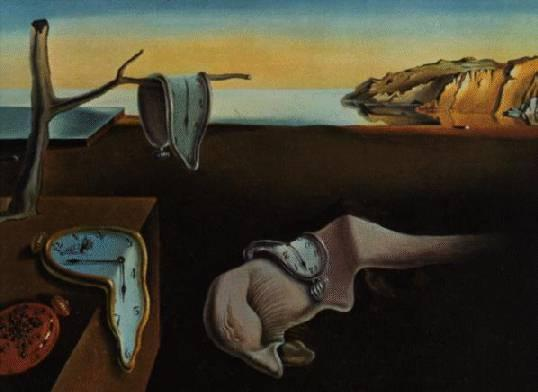
\includegraphics{jsslogo}
\caption{\label{fig:quine} Frequency distribution for number of days absent
from school.}
\end{figure}

























%% -- Summary/conclusions/discussion -------------------------------------------

\section{Summary and discussion} \label{sec:summary}

\begin{leftbar}
As usual \dots
\end{leftbar}

























%% -- Optional special unnumbered sections -------------------------------------

\section*{Computational details}

\begin{leftbar}
If necessary or useful, information about certain computational details
such as version numbers, operating systems, or compilers could be included
in an unnumbered section. Also, auxiliary packages (say, for visualizations,
maps, tables, \dots) that are not cited in the main text can be credited here.
\end{leftbar}

The results in this paper were obtained using
\proglang{R}~3.4.1 with the
\pkg{MASS}~7.3.47 package. \proglang{R} itself
and all packages used are available from the Comprehensive
\proglang{R} Archive Network (CRAN) at
\url{https://CRAN.R-project.org/}.


\section*{Acknowledgments}

\begin{leftbar}
All acknowledgments (note the AE spelling) should be collected in this
unnumbered section before the references. It may contain the usual information
about funding and feedback from colleagues/reviewers/etc. Furthermore,
information such as relative contributions of the authors may be added here
(if any).
\end{leftbar}


%% -- Bibliography -------------------------------------------------------------
%% - References need to be provided in a .bib BibTeX database.
%% - All references should be made with \cite, \citet, \citep, \citealp etc.
%%   (and never hard-coded). See the FAQ for details.
%% - JSS-specific markup (\proglang, \pkg, \code) should be used in the .bib.
%% - Titles in the .bib should be in title case.
%% - DOIs should be included where available.

\bibliography{../../bibliografia/Gaming/gaming}


%% -- Appendix (if any) --------------------------------------------------------
%% - After the bibliography with page break.
%% - With proper section titles and _not_ just "Appendix".

\newpage

\begin{appendix}











































































































\newpage

\section{Propiedades}\label{sec:propiedades}

Las siguientes tres propiedades, junto con las reglas del \emph{sum-product algorithm}, es lo \'unico que se necesita para calcular la posterior anal\'itica del modelo bayesiano.

\subsection*{Multiplicacion de normales}
\begin{equation}\label{eq:multiplicacion_normales}
\begin{split}
 \int_{-\infty}^{\infty} N(x|\mu_x,\sigma_x^2)N(x|\mu_y,\sigma_y^2) \, dx  &  \overset{*}{=} \int_{-\infty}^{\infty}  \underbrace{N(\mu_x|\mu_y,\sigma_x^2+\sigma_y^2)}_{\text{constante}} N(x|\mu_{*},\sigma_{*}^2) dx \\
 & = N(\mu_x|\mu_y,\sigma_x^2+\sigma_y^2) \underbrace{\int_{-\infty}^{\infty}  N(x|\mu_{*},\sigma_{*}^2) dx}_{1} \\
 & = N(\mu_x|\mu_y,\sigma_x^2+\sigma_y^2)
\end{split}
\end{equation}

Donde la igualdad destacada ($\overset{*}{=}$) se demuestra en la secci\'on~\ref{multiplicacion_normales} anexa.

\subsection*{Integrales con funci\'on indicadora}
\begin{equation}\label{eq:integral_con_indicadora}
\begin{split}
 \int_{-\infty}^{\infty}  \int_{-\infty}^{\infty}  \mathbb{I}(x=h(y,z)) f(x) g(y)\, dx\, dy &=  \int_{-\infty}^{\infty} \int_{h(y,z)}^{h(y,z)} f(h(y,z)) g(y)\, dx\, dy\\
 & = \int_{-\infty}^{\infty} f(h(y,z)) g(y) dy
 %& \propto \int f(h(y,z)) g(y) dy
\end{split}
\end{equation}

\subsection*{Simetr\'ia de normales}
\begin{equation}\label{eq:simetria}
 N(x|\mu,\sigma^2) = N(\mu|x,\sigma^2) = N(-\mu|-x,\sigma^2) = N(-x|-\mu,\sigma^2)
\end{equation}

\subsection*{Derivada de la acumulada normal}
\begin{equation}\label{eq:phi_norm}
 \frac{\partial}{\partial x} \Phi(x|\mu,\sigma^2) = N(x|\mu,\sigma^2)
\end{equation}

\subsection*{Distribuci\'on normal estandarizada}
\begin{equation}\label{eq:estandarizar}
 X \sim N(\mu,\sigma^2) \Rightarrow \frac{X-\mu}{\sigma} \sim N(0,1)
\end{equation}



\section{Ejemplo 2 vs 2}

\begin{figure}[t!]
  \centering
  \scalebox{.75}{\tikz{ %
        
      
        \node[factor] (fr) {} ;
        \node[const, right=of fr] (nfr) {$f_{r_1}$}; %
	
	\node[latent, above=of fr] (d) {$d_1$} ; %
        \node[factor, above=of d] (fd) {} ;
        \node[const, right=of fd] (nfd) {$f_{d_1}$}; %
	
        
        \node[latent, above=of fd,xshift=-0.75cm] (ta) {$t_a$} ; %
        \node[factor, left=of ta] (fta) {} ;
        \node[const, above=of fta] (nfta) {$f_{t_a}$}; %
        
        
        
        \node[latent, left=of fta,yshift=1cm] (p1) {$p_1$} ; %
        \node[factor, left=of p1] (fp1) {} ;
        \node[const, above=of fp1] (nfp1) {$f_{p_1}$}; %
        
        \node[latent, left=of fp1] (s1) {$s_1$} ; %
        \node[factor, left=of s1] (fs1) {} ;
	\node[const, above=of fs1] (nfs1) {$f_{s_1}$}; %
     
        \node[latent, left=of fta,yshift=-1cm] (p2) {$p_2$} ; %
        \node[factor, left=of p2] (fp2) {} ;
        \node[const, above=of fp2] (nfp2) {$f_{p_2}$}; %
        
        \node[latent, left=of fp2] (s2) {$s_2$} ; %
        \node[factor, left=of s2] (fs2) {} ;
	\node[const, above=of fs2] (nfs2) {$f_{s_2}$}; %
        
            
        \node[latent, above=of fd,xshift=0.75cm] (tb) {$t_b$} ; %
        \node[factor, right=of tb] (ftb) {} ;
        \node[const, above=of ftb] (nftb) {$f_{t_b}$}; %
        
        \node[latent, right=of ftb,yshift=1cm] (p3) {$p_3$} ; %
        \node[factor, right=of p3] (fp3) {} ;
        \node[const, above=of fp3] (nfp3) {$f_{p_3}$}; %
        
        \node[latent, right=of fp3] (s3) {$s_3$} ; %
        \node[factor, right=of s3] (fs3) {} ;
	\node[const, above=of fs3] (nfs3) {$f_{s_3}$}; %
     
        \node[latent, right=of ftb,yshift=-1cm] (p4) {$p_4$} ; %
        \node[factor, right=of p4] (fp4) {} ;
        \node[const, above=of fp4] (nfp4) {$f_{p_4}$}; %
        
        \node[latent, right=of fp4] (s4) {$s_4$} ; %
        \node[factor, right=of s4] (fs4) {} ;
	\node[const, above=of fs4] (nfs4) {$f_{s_4}$}; %
     
        \edge[-] {fr} {d};
	\edge[-] {d} {fd};
	
        \edge[-] {fd} {ta};
        \edge[-] {ta} {fta};
        \edge[-] {fta} {p1};
        \edge[-] {p1} {fp1};
        \edge[-] {fp1} {s1};
        \edge[-] {s1} {fs1};
        \edge[-] {fta} {p2};
        \edge[-] {p2} {fp2};
        \edge[-] {fp2} {s2};
        \edge[-] {s2} {fs2};
        	
	\edge[-] {fd} {tb};
        \edge[-] {tb} {ftb};
        \edge[-] {ftb} {p3};
        \edge[-] {p3} {fp3};
        \edge[-] {fp3} {s3};
        \edge[-] {s3} {fs3};
        \edge[-] {ftb} {p4};
        \edge[-] {p4} {fp4};
        \edge[-] {fp4} {s4};
        \edge[-] {s4} {fs4};
        
	
	\node[const, below=of nfr,xshift=7cm,yshift=-1cm] (dfr) { $fr_1 = \mathbb{I}(d_1>0)$}; %
	\node[const, left=of dfr,xshift=-0.5cm] (dfd) {$fd_1 = \mathbb{I}(d_1=t_a - t_b)$}; %
	\node[const, left=of dfd,xshift=-0.5cm] (dft) {$ft_e = \mathbb{I}(t_e = \sum_{i \in A_e} p_i)$}; %
        \node[const, left=of dft,xshift=-0.5cm] (dfp) {$fp_i = N(p_i;s_i,\beta^2)$}; %
        \node[const, left=of dfp,xshift=-0.5cm] (dfs) {$fs_i = N(s_i;\mu_i,\sigma^2)$}; %
 
	
	%\node[const, right= of r, xshift=1.2cm ,yshift=-2.1cm] (result-dist) {$r_{ab} \sim B\left(\Phi\left(\frac{\mu_a - \mu_b}{\sqrt{\beta_a^2+\beta_b^2}}\right)\right)$} ; %
	      
        }}
  \caption{\small Grafo bipartito de factorizaci\'on del modelo \texttt{TrueSkill} (Caso 2 vs 2)}
  \label{modelo_trueskill_2vs2}
\end{figure}


\subsection{Mensajes descendentes}

\paragraph{$\bm{m_{f_s \rightarrow s}(s)}:$}

\begin{equation}\label{eq:m_fs_s}
\begin{split}
 m_{f_{s_i} \rightarrow s_i}(s_i) & \overset{\hfrac{\text{eq}}{\ref{eq:m_f_v}}}{=} \int \dots \int f_{s_i}(\bm{x}) \prod_{h \in n(f_{s_i}) \setminus \{s_i\} } m_{h \rightarrow f_{s_i}}(h) d\bm{x}_{\setminus \{s_i\}}  \\
& \overset{\hfrac{\text{fig}}{\ref{modelo_trueskill_2vs2}}}{=} \int \dots \int N(s_i| \mu_i, \sigma_i^2) d\bm{x}_{\setminus \{s_i\} } \\
& \underset{*}{\overset{\hfrac{\text{eq}}{\ref{eq:m_f_v}}}{=}} N(s_i| \mu_i, \sigma_i^2)
\end{split}
\end{equation}

Notar que la igualdad se\~nalada $\overset{*}{=}$ vale por definici\'on de la notaci\'on resumen (Eq.~\ref{eq:m_f_v}),

\begin{equation*}
\begin{split}
\bm{x}_{\setminus \{s_i\} } & = \text{arg}(f) \setminus \{s_i\} \\
&= \text{arg}(N(s_i| \mu_i, \sigma_i^2)) \setminus \{s_i\} \\
&= \{s_i\} \setminus \{s_i\} \\
& = \emptyset
\end{split}
\end{equation*}



\paragraph{$\bm{m_{s \rightarrow f_p}(s)}:$}

\begin{equation}\label{eq:m_s_fp}
 m_{s_i \rightarrow f_{p_i}}(s_i) \overset{\hfrac{\text{eq}}{\ref{eq:m_v_f}}}{=} \prod_{g \in n(s_i) \setminus  \{f_{p_i} \}} m_{g \rightarrow s_i} (s_i) \overset{\hfrac{\text{fig}}{\ref{modelo_trueskill_2vs2}}}{=} m_{f_{s_i} \rightarrow s_i}(s_i) \overset{\hfrac{\text{eq}}{\ref{eq:m_fs_s}}}{=}   N(s_i| \mu_i, \sigma_i^2)
\end{equation}



\paragraph{$\bm{m_{f_p \rightarrow p}(p)}:$}

\begin{equation}\label{eq:m_fp_p}
\begin{split}
 m_{f_{p_i} \rightarrow p_i}(p_i) & \overset{\hfrac{\text{eq}}{\ref{eq:m_f_v}}}{=} \int \dots \int f_{p_i}(\bm{x}) \prod_{h \in n(f_{p_i}) \setminus \{p_i\} } m_{h \rightarrow f_{p_i}}(h) d\bm{x}_{\setminus \{p_i\} }  \\
 & \overset{\hfrac{\text{fig}}{\ref{modelo_trueskill_2vs2}}}{\underset{\hfrac{\text{eq}}{\ref{eq:m_s_fp}}}{=}} \int \dots \int N(p_i| s_i, \beta^2) N(s_i| \mu_i, \sigma_i^2) d\bm{x}_{\setminus \{p_i\} } \\[0.3cm]
 & \overset{\hfrac{\text{eq}}{\ref{eq:m_f_v}}}{=} \int N(p_i| s_i, \beta^2) N(s_i| \mu_i, \sigma_i^2) ds_i \\
 & \overset{\hfrac{\text{eq}}{\ref{eq:simetria}}}{=} \int N(s_i|p_i, \beta^2) N(s_i| \mu_i, \sigma_i^2) ds_i \\
& \overset{\hfrac{\text{eq}}{\ref{eq:multiplicacion_normales}}}{=} N(p_i|\mu_i,\beta^2 + \sigma_i^2)
\end{split}
\end{equation}

\paragraph{$\bm{m_{p \rightarrow f_t}(p)}:$}

\begin{equation}\label{eq:m_p_ft}
\begin{split}
 m_{p_i \rightarrow f_{t_e}}(p_i) & \overset{\hfrac{\text{eq}}{\ref{eq:m_v_f}}}{=} \prod_{g \in n(p_i) \setminus  \{f_{t_e} \}} m_{g \rightarrow p_i} (p_i) \\
 & \overset{\hfrac{\text{fig}}{\ref{modelo_trueskill_2vs2}}}{=} m_{f_{p_i} \rightarrow p_i}(p_i) \overset{\hfrac{\text{eq}}{\ref{eq:m_fp_p}}}{=} N(p_i|\mu_i,\beta^2 + \sigma_i^2)
\end{split}
\end{equation}

\paragraph{$\bm{m_{f_t \rightarrow t}(t)}:$}

\begin{equation}
\begin{split}
 m_{f_{t_e} \rightarrow t_e}(t_e) & \overset{\hfrac{\text{eq}}{\ref{eq:m_f_v}}}{=} \int \dots \int f_{t_e}(\bm{x}) \prod_{h \in n(f_{t_e}) \setminus \{t_e\} } m_{h \rightarrow f_{t_e}}(h) d\bm{x}_{\setminus \{t_e\} }  \\
 & \overset{\hfrac{\text{fig}}{\ref{modelo_trueskill_2vs2}}}{\underset{\hfrac{\text{eq}}{\ref{eq:m_p_ft}}}{=}} \int \dots \int \mathbb{I}(t_e = p_i + p_j) N(p_i|\mu_i,\beta^2 + \sigma_i^2)N(p_j|\mu_j,\beta^2 + \sigma_j^2) d\bm{x}_{\setminus \{t_e\} }\\[0.3cm]
 & \overset{\hfrac{\text{eq}}{\ref{eq:m_f_v}}}{=} \iint \mathbb{I}(t_e = p_i + p_j) N(p_i|\mu_i,\beta^2 + \sigma_i^2)N(p_j|\mu_j,\beta^2 + \sigma_j^2) dp_idp_j \\
 & \overset{\hfrac{\text{eq}}{\ref{eq:integral_con_indicadora}}}{=} \int N(p_i|\mu_i,\beta^2 + \sigma_i^2) N(t_e - p_i|\mu_j,\beta^2 + \sigma_j^2) dp_i   \\
 & \overset{\hfrac{\text{eq}}{\ref{eq:simetria}}}{=} \int N(p_i|\mu_i,\beta^2 + \sigma_i^2) N(p_i|t_e - \mu_j,\beta^2 + \sigma_j^2) dp_i \\
 & \overset{\hfrac{\text{eq}}{\ref{eq:multiplicacion_normales}}}{=} N(t_e|\mu_i+\mu_j,2\beta^2 + \sigma_i^2 + \sigma_j^2)
\end{split}
\end{equation}

\vspace{0.3cm}

General (por inducci\'on)
\begin{equation}\label{eq:m_ft_t}
 m_{f_{t_e} \rightarrow t_e}(t_e) =  N \Big( t_e | \underbrace{\sum_{i\in A_e } \mu_i}_{\hfrac{\text{Habilidad}}{\text{de equipo}} \ \mu_e}, \underbrace{\sum_{i \in A_e} \beta^2 + \sigma_i^2}_{\hfrac{\text{Varianza}}{\text{de equipo}} \ \sigma_e^2} \Big) = N(t_e | \mu_e, \sigma_e^2)
\end{equation}

Ver anexo~\ref{suma_normales_induccion}, la secci\'on sobre suma de $n$ normales.

\paragraph{$\bm{m_{t \rightarrow f_d}(t)}:$}

\begin{equation}\label{eq:m_t_fd}
\begin{split}
m_{t_e \rightarrow f_{d_{k}}}(d_{k}) & \overset{\hfrac{\text{eq}}{\ref{eq:m_v_f}}}{=} \prod_{g \in n(t_e) \setminus  \{f_{d_{k}} \}} m_{g \rightarrow t_e} (t_e) \\[0.3cm]
 & \overset{\hfrac{\text{fig}}{\ref{modelo_trueskill_2vs2}}}{=} m_{f_{t_e} \rightarrow t_e}(t_e) \overset{\hfrac{\text{eq}}{\ref{eq:m_ft_t}}}{=} N(t_e| \sum_{i \in A_e} \mu_i, \sum_{i \in A_e} \beta^2 + \sigma_i^2) \overset{\hfrac{\text{eq}}{\ref{eq:m_ft_t}}}{=} N(t_e|\mu_e,\sigma_e^2)
\end{split}
\end{equation}

\paragraph{$\bm{m_{f_d \rightarrow d}(d)}:$}

\begin{equation}
 \begin{split}
  m_{f_{d_1} \rightarrow d_1}(d_1) & \overset{\hfrac{\text{eq}}{\ref{eq:m_f_v}}}{=} \int \dots \int f_{d_1}(\bm{x}) \prod_{h \in n(f_{d_1}) \setminus \{d_1\} } m_{h \rightarrow f_{d_1}}(h) \, d\bm{x}_{\setminus \{d_1\} }  \\
  & \overset{\hfrac{\text{fig}}{\ref{modelo_trueskill_2vs2}}}{\underset{\hfrac{\text{eq}}{\ref{eq:m_t_fd}}}{=}} \int \int \mathbb{I}(d_1 = t_a - t_b) N(t_a| \mu_a, \sigma_a^2)  N(t_b| \mu_b, \sigma_b^2)  dt_adt_b \\[0.25cm]
  & \overset{\hfrac{\text{eq}}{\ref{eq:integral_con_indicadora}}}{=} \int N(d_1 + t_b| \mu_a, \sigma_a^2)  N(t_b| \mu_a, \sigma_b^2)  dt_b \\
  & \overset{\hfrac{\text{eq}}{\ref{eq:simetria}}}{=} \int N(t_b| \mu_a - d_1 , \sigma_a^2)  N(t_b| \mu_b, \sigma_b^2)  dt_b \\
  & \overset{\hfrac{\text{eq}}{\ref{eq:multiplicacion_normales}}}{=} N( \mu_a - d_1 | \mu_b, \sigma_a^2 +\sigma_b^2  ) \\
  & \overset{\hfrac{\text{eq}}{\ref{eq:simetria}}}{=} N( d_1 | \mu_a - \mu_b, \sigma_a^2 +\sigma_b^2  )
 \end{split}
\end{equation}

General

\begin{equation} \label{eq:m_fd_d}
 m_{f_{d_1} \rightarrow d_1}(d_1) = N\Bigg(d_1 \ | \ \underbrace{\sum_{i \in A_a} \mu_i - \sum_{i \in A_b} \mu_i}_{\hfrac{\text{Diferencia}}{\text{esperada}} \, (\delta)} \ , \  \underbrace{\sum_{i \in A_a \cup A_b} \beta^2 + \sigma_i^2}_{\hfrac{\text{Varianza}}{\text{total}} \, (\vartheta) } \Bigg) = N(d_1 | \delta, \vartheta)
\end{equation}

\paragraph{$\bm{m_{d \rightarrow f_r}(r)}:$}

\begin{equation}\label{eq:m_d_fr}
\begin{split}
m_{d \rightarrow f_r}(d) & \overset{\hfrac{\text{eq}}{\ref{eq:m_v_f}}}{=} \prod_{g \in n(t_e) \setminus  \{f_{d_{k}} \}} m_{g \rightarrow t_e} (t_e) \\[0.3cm]
 & \overset{\hfrac{\text{fig}}{\ref{modelo_trueskill_2vs2}}}{=} m_{f_d \rightarrow d}(d) \overset{\hfrac{\text{eq}}{\ref{eq:m_fd_d}}}{=} N(d_1| \delta, \vartheta)
\end{split}
\end{equation}

\paragraph{$\bm{m_{f_r \rightarrow r}(r)}:$} (Caso ganador)

\begin{equation}\label{eq:m_fr_r}
\begin{split}
 m_{f_{r_1} \rightarrow r_1}(r_1) & \overset{\hfrac{\text{eq}}{\ref{eq:m_f_v}}}{=} \int \dots \int f_{r_1}(\bm{x}) \prod_{h \in n(f_{r_1}) \setminus \{r_1\} } m_{h \rightarrow f_{r_1}}(h) \, d\bm{x}_{\setminus \{r_1\} }  \\[0.2cm]
 & \overset{\hfrac{\text{fig}}{\ref{modelo_trueskill_2vs2}}}{\underset{\hfrac{\text{eq}}{\ref{eq:m_d_fr}}}{=}} \int \mathbb{I}(d_1 > 0) N(d_1 | \delta, \vartheta)  dd_1 \\[0.2cm]
 &  \overset{\hfrac{\text{eq}}{\ref{eq:estandarizar}}}{=} \int \mathbb{I}(d_1 > 0) N( \frac{d_1 - \delta}{\vartheta}) dd_1 \\[0.2cm]
 & = 1 - \Phi(\frac{-\delta}{\vartheta}) \\
 & = \Phi(\frac{\delta}{\vartheta})
\end{split}
\end{equation}













\subsubsection{Mensajes ascendentes}

\paragraph{$\bm{m_{f_r \rightarrow d}(d)}:$}

\begin{equation}\label{eq:m_fr_d}
\begin{split}
m_{f_r \rightarrow d_1}(d_1) & \overset{\hfrac{\text{fig}}{\ref{modelo_trueskill_2vs2}}}{\underset{\hfrac{\text{eq}}{\ref{eq:m_f_v}}}{=}} \mathbb{I}(d_1 > 0)
\end{split}
\end{equation}


\paragraph{$\bm{m_{d \rightarrow f_d}(d)}:$}
\begin{equation}\label{eq:m_d_fd}
\begin{split}
m_{d_1 \rightarrow f_{d_1}}(d_1) & \overset{\hfrac{\text{eq}}{\ref{eq:m_v_f}}}{=} \prod_{g \in n(d_1) \setminus  \{f_{d_1} \}} m_{g \rightarrow d_1} (d_1) \\[0.3cm]
 & \overset{\hfrac{\text{fig}}{\ref{modelo_trueskill_2vs2}}}{=} m_{f_r \rightarrow d_1}(d_1) \overset{\hfrac{\text{eq}}{\ref{eq:m_fr_d}}}{=} \mathbb{I}(d_1 > 0)
\end{split}
\end{equation}

\paragraph{$\bm{m_{f_{d_1} \rightarrow t_a}(t_a)}:$} (Caso ganador)
\begin{equation}\label{eq:m_fd_ta}
\begin{split}
m_{f_{d_1} \rightarrow t_a}(t_a) & \overset{\hfrac{\text{eq}}{\ref{eq:m_f_v}}}{=} \int \dots \int f_{d_1}(\bm{x}) \prod_{h \in n(f_{d_1}) \setminus \{t_a\} } m_{h \rightarrow f_{d_1}}(h) \, d\bm{x}_{\setminus \{t_a\} }  \\
&\overset{\hfrac{\text{fig}}{\ref{modelo_trueskill_2vs2}}}{\underset{\hfrac{\text{eq}}{\ref{eq:m_t_fd}}}{=}}  \int \dots \int \mathbb{I}(d_1 = t_a - t_b) \mathbb{I}(d_1 > 0) N(t_b | \mu_b , \sigma_b^2 )  \, d\bm{x}_{\setminus \{t_a\} } \\[0.1cm]
& \overset{\hfrac{\text{eq}}{\ref{eq:m_f_v}}}{=} \iint \mathbb{I}(d_1 = t_a - t_b) \mathbb{I}(d_1 > 0) N(t_b | \mu_b , \sigma_b^2 ) \, dd_1\,dt_b \\
& \overset{\hfrac{\text{eq}}{\ref{eq:integral_con_indicadora}}}{=} \int \mathbb{I}( t_a > t_b)  N(t_b | \mu_b , \sigma_b^2 ) \,dt_b  \\
& \overset{\hfrac{\text{fig}}{\ref{fig:m_fd_t}}}{=} \Phi (t_a| \mu_b, \sigma_b^2)  \overset{\hfrac{\mu_b}{\sigma_b}}{=}  \Phi \Big(t_a| \sum_{i \in A_b} \mu_i , \sum_{i \in A_b} \beta^2 + \sigma_i^2 \Big)
\end{split}
\end{equation}

\paragraph{$\bm{m_{f_{d_1} \rightarrow t_b}(t_b)}:$} (Caso perdedor)
\begin{equation}\label{eq:m_fd_tb}
\begin{split}
m_{f_{d_1} \rightarrow t_b}(t_b) &\overset{\hfrac{\text{eq}}{\ref{eq:m_f_v}}}{=} \int \dots \int f_{d_1}(\bm{x}) \prod_{h \in n(f_{d_1}) \setminus \{t_b\} } m_{h \rightarrow f_{d_1}}(h) \, d\bm{x}_{\setminus \{t_a\} }  \\
&\overset{\hfrac{\text{fig}}{\ref{modelo_trueskill_2vs2}}}{\underset{\hfrac{\text{eq}}{\ref{eq:m_t_fd}}}{=}}  \int \dots \int \mathbb{I}(d_1 = t_a - t_b) \mathbb{I}(d_1 > 0) N(t_a | \mu_a , \sigma_a^2 )  \, d\bm{x}_{\setminus \{t_b\} } \\[0.1cm]
&\overset{\hfrac{\text{eq}}{\ref{eq:m_f_v}}}{=} \iint \mathbb{I}(d_1 = t_a - t_b) \mathbb{I}(d_1 > 0)  N(t_a | \mu_a , \sigma_a^2 )  \, dd_1\,dt_a \\
&\overset{\hfrac{\text{eq}}{\ref{eq:integral_con_indicadora}}}{=} \int \mathbb{I}( t_a > t_b)   N(t_a | \mu_a , \sigma_a^2 ) \,dt_a \\
&\overset{\hfrac{\text{fig}}{\ref{fig:m_fd_t}}}{=} 1 - \Phi (t_b| \mu_a , \sigma_a^2 ) \overset{\hfrac{\mu_a}{\sigma_a}}{=} 1 - \Phi \Big(t_b| \sum_{i \in A_a} \mu_i , \sum_{i \in A_a} \beta^2 + \sigma_i^2 \Big)
\end{split}
\end{equation}

\begin{figure}[t!]
\centering
  \begin{subfigure}[t]{0.48\textwidth}
  \includegraphics[width=\textwidth]{figures/m_d_ta.pdf}
  \caption{$m_{f_{d_1} \rightarrow t_a}(t_a)$: (Caso ganador)}
  \label{fig:m_fd_ta}
  \end{subfigure}
  \begin{subfigure}[t]{0.48\textwidth}
  \includegraphics[width=\textwidth]{figures/m_d_tb.pdf}
  \caption{$m_{f_{d_1} \rightarrow t_b}(t_b)$: (Caso perdedor)}
  \label{fig:m_fd_tb}
  \end{subfigure}
  \caption{Notar que en el caso ganador, $t_a$ es un valor fijo que entra como par\'ametro en la funci\'on $m_{f_{d_1} \rightarrow t_a}(t_a)$. El caso perdedor es an\'alogo.}
  \label{fig:m_fd_t}
\end{figure}

\paragraph{$\bm{m_{t_a \rightarrow f_{t_a}}(t_a)}:$} (Caso ganador)

\begin{equation}\label{eq:m_ta_ft}
\begin{split}
 m_{t_a \rightarrow f_{t_a}}(t_a) \overset{\hfrac{\text{eq}}{\ref{eq:m_v_f}}}{=} \prod_{g \in n(t_a) \setminus  \{f_{t_a} \}} m_{g \rightarrow t_a} (t_a)  \overset{\hfrac{\text{eq}}{\ref{eq:m_fd_ta}}}{=} \Phi(t_a|\mu_b,\sigma_b^2) \overset{\hfrac{\mu_b}{\sigma_b}}{=} \Phi \Big(t_a| \sum_{i \in A_b} \mu_i , \sum_{i \in A_b} \beta^2 + \sigma_i^2 \Big)
\end{split}
\end{equation}

\paragraph{$\bm{m_{t_b \rightarrow f_{t_b}}(t_b)}:$} (Caso perdedor)
\begin{equation}\label{eq:m_tb_ft}
\begin{split}
 m_{t_b \rightarrow f_{t_b}}(t_b) \overset{\hfrac{\text{eq}}{\ref{eq:m_v_f}}}{=} \prod_{g \in n(t_b) \setminus  \{f_{t_b} \}} m_{g \rightarrow t_b} (t_b)  \overset{\hfrac{\text{eq}}{\ref{eq:m_fd_tb}}}{=} 1- \Phi(t_b|\mu_a,\sigma_a^2) \overset{\hfrac{\mu_a}{\sigma_a}}{=} 1 - \Phi \Big(t_b| \sum_{i \in A_a} \mu_i , \sum_{i \in A_a} \beta^2 + \sigma_i^2 \Big)
\end{split}
\end{equation}



\paragraph{$\bm{m_{f_{t_a} \rightarrow p_1}(p_1)}:$} (Caso ganador)
\begin{equation}\label{eq:m_fta_p_inicial}
\begin{split}
m_{f_{t_a} \rightarrow p_1}(p_1)  &\overset{\hfrac{\text{eq}}{\ref{eq:m_f_v}}}{=} \int \dots \int f_{t_a}(\bm{x}) \prod_{h \in n(f_{t_a}) \setminus \{p_1\} } m_{h \rightarrow f_{t_a}}(h) \, d\bm{x}_{\setminus \{p_1\} }  \\
&\overset{\hfrac{\text{fig}}{\ref{modelo_trueskill_2vs2}}}{\underset{\hfrac{\text{eq}}{\ref{eq:m_ta_ft}}}{=}} \int \dots \int \mathbb{I}( t_a = p_1 + p_2) N(p_2| \mu_2, \beta^2 + \sigma_2^2 ) \, \Phi (t_a| \mu_b , \sigma_b^2 ) \, d\bm{x}_{\setminus \{p_1\} }\\[0.1cm]
&\overset{\hfrac{\text{eq}}{\ref{eq:m_f_v}}}{=} \iint \mathbb{I}( t_a = p_1 + p_2) \, N(p_2| \mu_2, \beta^2 + \sigma_2^2 ) \, \Phi (t_a| \mu_b , \sigma_b^2 ) \, dt_a dp_2 \\
&\overset{\hfrac{\text{eq}}{\ref{eq:integral_con_indicadora}}}{=} \int  \, N(p_2| \mu_2, \beta^2 + \sigma_2^2 ) \, \Phi (p_1 + p_2| \mu_b , \sigma_b^2 ) \, dp_2 \\
&\overset{\hfrac{\text{eq}}{\ref{eq:simetria}}}{=} \int  N(p_2| \mu_2, \beta^2 + \sigma_2^2 ) \, \Phi (p_1 | \mu_b - p_2 , \sigma_b^2) \, dp_2 \\
&= \kappa(p_1)
\end{split}
\end{equation}

La derivada de la funci\'on de distribuci\'on acumulada $\Phi(\,)$ es el valor de la densidad de la funci\'on de probabilidad $N(\,)$. Con esta idea en mente, tomamos la derivada de ambos lados de la igualdad:

\begin{equation}\label{eq:ta-p_derivada}
\begin{split}
\frac{\partial\kappa(x)}{\partial x} &= \frac{\partial}{\partial x} \int  N(y| \mu_y, \sigma_y^2 ) \,   \Phi (x | \mu_x -y , \sigma_x^2 ) \, dy \\
&= \int  N(y| \mu_y, \sigma_y^2 ) \, \frac{\partial}{\partial x} \,\Phi (x| \mu_x - y, \sigma_x^2 )  \, dy   \\
& \overset{\hfrac{\text{eq}}{\ref{eq:phi_norm}}}{=} \int  N(y| \mu_y, \sigma_y^2 ) \, N(x| \mu_x -y , \sigma_x^2)  \, dy  \\
& \overset{\hfrac{\text{eq}}{\ref{eq:simetria}}}{=} \int  N(y| \mu_y, \sigma_y^2 ) \, N(y| \mu_x  -x , \sigma_x^2)  \, dy  \\
&\overset{\hfrac{\text{eq}}{\ref{eq:multiplicacion_normales}}}{\underset{\hfrac{\text{eq}}{\ref{eq:simetria}}}{=}} N(x| \mu_x - \mu_y, \sigma_x^2 + \sigma_y^2)
\end{split}
\end{equation}

Luego

\begin{equation}\label{eq:m_fta_p}
 m_{f_{t_a} \rightarrow p_1}(p_1) \overset{\hfrac{\text{eq}}{\ref{eq:m_fta_p_inicial}}}{\underset{\hfrac{\text{eq}}{\ref{eq:ta-p_derivada}}}{=}}  \Phi(p_1| \mu_b - \mu_2, \beta^2 + \sigma_2^2 + \sigma_b^2)  \overset{\hfrac{\mu_b}{\sigma_b}}{=}  \Phi\Big(p_1| \sum_{i \in A_b} \mu_i - \mu_2, \beta^2 + \sigma_2^2 + \sum_{i \in A_b} \beta^2 + \sigma_i^2 \Big)
\end{equation}

\paragraph{$\bm{m_{f_{t_b} \rightarrow p_3}(p_3)}:$} (Caso perdedor)
\begin{equation}\label{eq:m_ftb_p}
\begin{split}
m_{f_{t_b} \rightarrow p_3}(p_3)&\overset{\hfrac{\text{eq}}{\ref{eq:m_f_v}}}{=} \int \dots \int f_{t_a}(\bm{x}) \prod_{h \in n(f_{t_a}) \setminus \{p_1\} } m_{h \rightarrow f_{t_a}}(h) \, d\bm{x}_{\setminus \{p_1\} }  \\
&\overset{\hfrac{\text{fig}}{\ref{modelo_trueskill_2vs2}}}{\underset{\hfrac{\text{eq}}{\ref{eq:m_tb_ft}}}{=}} \int \dots \int \mathbb{I}( t_b = p_3 + p_4) \, (1-\Phi (t_b| \mu_a , \sigma_a^2 )) \, N(p_4| \mu_4, \beta^2 + \sigma_4^2 ) \, d\bm{x}_{\setminus \{p_3\} }\\[0.1cm]
&\overset{\hfrac{\text{eq}}{\ref{eq:m_f_v}}}{=} \iint \mathbb{I}( t_b = p_3 + p_4) N(p_4| \mu_4, \beta^2 + \sigma_4^2 )  (1 - \Phi (t_b| \mu_a , \sigma_a^2) )\, dt_b dp_4 \\
&\overset{\hfrac{\text{eq}}{\ref{eq:integral_con_indicadora}}}{\underset{\hfrac{\text{eq}}{\ref{eq:simetria}}}{=}} \int N(p_4| \mu_4, \beta^2 + \sigma_4^2 )  (1 - \Phi (p_3 | \mu_a - p_4 , \sigma_a^2 ) ) \,  dp_4 \\
& =  \underbrace{\int N(p_4| \mu_4, \beta^2 + \sigma_4^2 )dp_4}_{1}  -  \underbrace{\int N(p_4| \mu_4, \beta^2 + \sigma_4^2 ) \Phi (p_3 | \mu_a - p_4 , \sigma_a^2 ) ) \, dp_4}_{\kappa(p_3)} \\
&\overset{\hfrac{\text{eq}}{\ref{eq:ta-p_derivada}}}{=} 1 - \Phi(p_3, \mu_a  - \mu_4, \beta^2 + \sigma_4^2 + \sigma_a^2)\\[0.1cm]
&\overset{\hfrac{\mu_a}{\sigma_a}}{=} 1 - \Phi\Big(p_3, \sum_{i \in A_a} \mu_i  - \mu_4, \beta^2 + \sigma_4^2 + \sum_{i \in A_a} \beta^2 + \sigma_i^2  \Big)
\end{split}
\end{equation}

\paragraph{$\bm{m_{p_1 \rightarrow f_{p_1}}(s_1)}:$} (Caso ganador)

\begin{equation}\label{eq:m_p1_fp}
\begin{split}
 m_{p_1 \rightarrow f_{p_1}}(p_1) \overset{\hfrac{\text{eq}}{\ref{eq:m_v_f}}}{=} \prod_{g \in n(p_1) \setminus  \{f_{p_1} \}} m_{g \rightarrow p_1} (p_1)  \overset{\hfrac{\text{eq}}{\ref{eq:m_fta_p}}}{=}  \Phi(p_1| \mu_b - \mu_2, \beta^2 + \sigma_2^2 + \sigma_b^2)
\end{split}
\end{equation}


\paragraph{$\bm{m_{p_3 \rightarrow f_{p_3}}(s_1)}:$} (Caso perdedor)

\begin{equation}\label{eq:m_p3_fp}
\begin{split}
 m_{p_3 \rightarrow f_{p_3}}(p_3) \overset{\hfrac{\text{eq}}{\ref{eq:m_v_f}}}{=} \prod_{g \in n(p_3) \setminus  \{f_{p_3} \}} m_{g \rightarrow p_3} (p_3)  \overset{\hfrac{\text{eq}}{\ref{eq:m_ftb_p}}}{=}  1 - \Phi(p_3, \mu_a  - \mu_4, \beta^2 + \sigma_4^2 + \sigma_a^2)
\end{split}
\end{equation}

\paragraph{$\bm{m_{f_{p_1} \rightarrow s_1}(s_1)}:$} (Caso ganador)
\begin{equation}\label{eq:m_fp_s1}
\begin{split}
m_{f_{p_1} \rightarrow s_1}(s_1) & \overset{\hfrac{\text{eq}}{\ref{eq:m_f_v}}}{=} \int \dots \int f_{p_1}(\bm{x}) \prod_{h \in n(f_{p_1}) \setminus \{s_1\} } m_{h \rightarrow f_{p_1}}(h) \, d\bm{x}_{\setminus \{s_1\} }  \\
&\overset{\hfrac{\text{fig}}{\ref{modelo_trueskill_2vs2}}}{\underset{\hfrac{\text{eq}}{\ref{eq:m_p1_fp}}}{=}} \int \dots \int N(p_1| s_1, \beta^2) \, \Phi(p_1| \mu_b - \mu_2, \beta^2 + \sigma_2^2 + \sigma_b^2 ) \, d\bm{x}_{\setminus \{s_1\} }
\\[0.1cm]
& \overset{\hfrac{\text{eq}}{\ref{eq:m_f_v}}}{\underset{\hfrac{\text{eq}}{\ref{eq:simetria}}}{=}} \int N(p_1| s_1, \beta^2) \, \Phi(\mu_2| \mu_b -  p_1, \beta^2 + \sigma_2^2 + \sigma_b^2) \, dp_1 \\[0.1cm]
&\overset{\hfrac{\text{eq}}{\ref{eq:ta-p_derivada}}}{=} \Phi(s_1| \mu_b - \mu_2, 2\beta^2 + \sigma_2^2 + \sigma_b^2)
\end{split}
\end{equation}

General (N vs N)
\begin{equation}\label{eq:m_fp_s1_gral}
\begin{split}
m_{f_{p_1} \rightarrow s_1}(s_1) & \overset{\hfrac{\text{eq}}{\ref{eq:m_fp_s1}}}{=} \Phi(s_1| \mu_b - \mu_a + \mu_1, \sigma_b^2 +\sigma_a^2 - \sigma_1^2 )  \\
& \overset{\hfrac{\mu_b}{\sigma_b}}{=} \Phi\Big(s_1| \underbrace{\sum_{i \in A_b} \mu_i - \sum_{i \in A_a} \mu_i }_{-\hfrac{\text{Diferencia}}{\text{esperada}} \, -\delta = \delta } + \mu_1 , \underbrace{\sum_{i \in A_b \cup A_a} \beta^2 + \sigma_i^2}_{\hfrac{\text{Varianza}}{\text{total}} \, \vartheta^2} - \sigma_1^2   \Big) \\
& \overset{\hfrac{\delta}{\vartheta}}{=} \Phi(s_1|-\delta + \mu_1,\vartheta^2-\sigma_1^2) \\
& \overset{\hfrac{\text{eq}}{\ref{eq:simetria}}}{=} 1- \Phi(0| \underbrace{\delta - \mu_1 + s_1}_{\hfrac{\text{Diferencia esperada}}{\text{parametrizada}} \, \delta_1(s_1)},\underbrace{\vartheta^2-\sigma_1^2}_{\vartheta_1^2}) \\
& \overset{\hfrac{\delta_1}{\vartheta_1}}{=} 1- \Phi(0|\delta_1(s_1),\vartheta_1^2) \\
&\overset{\hfrac{\text{eq}}{\ref{eq:estandarizar}}}{=} 1- \Phi\Big(\frac{0-\delta_1(s_1)}{\vartheta_1}\Big)\\
&\overset{\hfrac{\text{eq}}{\ref{eq:simetria}}}{=} \Phi\Big(\frac{\delta_1(s_1)}{\vartheta_1}\Big)
\end{split}
\end{equation}

\textbf{Nota}: el mensaje $m_{f_{p_1} \rightarrow s_1}(s_1)$ computa la ``probabilidad de ganar parametrizada'', esto es la probabilidad de ganar si conoci\'eramos la habilidad del jugador. Si conocemos la habilidad del jugador entonces hay que eliminar la varianza de la distribuci\'on de creencias de la varianza total (lo que hacemos en $\vartheta_1$) y hay que remplazar la media de la distribuci\'on de creencias por la verdadera habilidad en la diferencia esperada (lo que hacemos en $\delta_1(s_1)$).

\paragraph{$\bm{m_{f_{p_3} \rightarrow s_3}(s_3)}:$}

\begin{equation}\label{eq:m_fp_s3}
\begin{split}
m_{f_{p_3} \rightarrow s_3}(s_3) & \overset{\hfrac{\text{eq}}{\ref{eq:m_f_v}}}{=} \int \dots \int f_{p_3}(\bm{x}) \prod_{h \in n(f_{p_3}) \setminus \{s_3\} } m_{h \rightarrow f_{p_3}}(h) \, d\bm{x}_{\setminus \{s_3\} }  \\
&\overset{\hfrac{\text{fig}}{\ref{modelo_trueskill_2vs2}}}{\underset{\hfrac{\text{eq}}{\ref{eq:m_p3_fp}}}{=}} \int \dots \int N(p_3| s_3, \beta^2) (1 - \Phi(p_3, \mu_a  - \mu_4, \beta^2 + \sigma_4^2 + \sigma_a^2)) \, d\bm{x}_{\setminus \{s_3\} }\\
& \overset{\hfrac{\text{eq}}{\ref{eq:m_f_v}}}{\underset{\hfrac{\text{eq}}{\ref{eq:simetria}}}{=}} \int N(p_3| s_3, \beta^2) (1 - \Phi(\mu_4, \mu_a  - p_3, \beta^2 + \sigma_4^2 + \sigma_a^2)) \, dp_3 \\
&=\int N(p_3| s_3, \beta^2) \, dp_3 -  \int N(p_3| s_3, \beta^2)  \Phi(\mu_4, \mu_a  - p_3, \beta^2 + \sigma_4^2 + \sigma_a^2) \, dp_3 \\
&\overset{\hfrac{\text{eq}}{\ref{eq:ta-p_derivada}}}{=} 1 - \Phi\Big(s_3| \mu_a-  \mu_4, 2\beta^2 + \sigma_4^2 + \sigma_a^2 \Big)
\end{split}
\end{equation}

General (N vs N)

\begin{equation}
\begin{split}
m_{f_{p_3} \rightarrow s_3}(s_3) & \overset{\hfrac{\text{eq}}{\ref{eq:m_fp_s3}}}{=} 1 - \Phi\Big(s_3| \underbrace{\mu_a-\mu_b}_{\delta}+\mu_3, \underbrace{\sigma_a^2 + \sigma_b^2}_{\vartheta^2} - \sigma_3^2 \Big) \\
& \overset{\hfrac{\delta}{\vartheta}}{=} 1 - \Phi\Big(s_3| \delta +\mu_3, \vartheta^2- \sigma_3^2 \Big) \overset{\hfrac{\text{eq}}{\ref{eq:simetria}}}{=} \Phi\Big(0| \underbrace{-\delta-\mu_3+s_3}_{\delta_3(s_3)}, \underbrace{\vartheta^2- \sigma_3^2}_{\vartheta_3^2} \Big) \\
& \overset{\hfrac{\delta_3}{\vartheta_3}}{=} \Phi(0|\delta_3(s_3),\vartheta_3^2)  \overset{\hfrac{\text{eq}}{\ref{eq:estandarizar}}}{=}  \Phi\left(\frac{0-\delta_3(s_3)}{\vartheta_3}\right) \\
& \overset{\hfrac{\text{eq}}{\ref{eq:simetria}}}{=} \Phi\Big(\frac{-\delta_3(s_3)}{\vartheta_3}\Big)
\end{split}
\end{equation}

\textbf{Nota}: el mensaje $m_{f_{p_3} \rightarrow s_3}(s_3)$ computa la ``probabilidad de perder parametrizada'' (que es la misma que la probabilidad de ganar de su contrincante). Si conoci\'eramos la habilidad del jugador entonces hay que eliminar la varianza de la distribuci\'on de creencias de la varianza total (lo que hacemos en $\vartheta_3$) y hay que remplazar la media de la distribuci\'on de creencias por la verdadera habilidad en la diferencia esperada (lo que hacemos en $\delta_3(s_3)$).

\subsubsection{Posterior ganador y perdedor}
\paragraph{Ganador}
\begin{equation}\label{eq:posterior_ganador}
 p(s_1|o,A) \overset{\hfrac{\text{eq}}{\ref{eq:marginal}}}{=} \prod_{h \in n(x_i)} m_{h \rightarrow x_i} \overset{\hfrac{\text{fig}}{\ref{modelo_trueskill_2vs2}}}{\underset{\hfrac{\text{eq}}{\ref{eq:m_fp_s1_gral}}}{=}}  N(s_1| \mu_1, \sigma_1^2)  \Phi\left(\frac{\delta_1(s_1)}{\vartheta_1}\right)
\end{equation}


\begin{figure}[t!]
\centering
  \begin{subfigure}[t]{0.48\textwidth}
  \includegraphics[page=1,width=\textwidth]{figures/posterior_ganador.pdf}
  \caption{}
  \label{posterior_ganador_image}
  \end{subfigure}
  \begin{subfigure}[t]{0.48\textwidth}
  \includegraphics[page=2,width=\textwidth]{figures/posterior_ganador.pdf}
  \caption{}
  \label{posterior_ganador_distribution}
  \end{subfigure}
  \caption{Posterior ganador}
  \label{posterior_ganador}
\end{figure}

\paragraph{Perdedor}

\begin{equation}\label{eq:posterior_perdedor}
 p(s_1|o,A) \overset{\hfrac{\text{eq}}{\ref{eq:marginal}}}{=} \prod_{h \in n(x_i)} m_{h \rightarrow x_i} \overset{\hfrac{\text{fig}}{\ref{modelo_trueskill_2vs2}}}{\underset{\hfrac{\text{eq}}{\ref{eq:m_fp_s1_gral}}}{=}}  N(s_1| \mu_1, \sigma_1^2)  \Phi\left(\frac{-\delta_1(s_1)}{\vartheta_1}\right)
\end{equation}


\begin{figure}[t!]
\centering
  \begin{subfigure}[t]{0.48\textwidth}
  \includegraphics[page=1,width=\textwidth]{figures/posterior_perdedor.pdf}
  \caption{}
  \label{posterior_perdedor_image}
  \end{subfigure}
  \begin{subfigure}[t]{0.48\textwidth}
  \includegraphics[page=2,width=\textwidth]{figures/posterior_perdedor.pdf}
  \caption{}
  \label{posterior_perdedor_distribution}
  \end{subfigure}
  \caption{Posterior perdedor}
  \label{posterior_perdedor}
\end{figure}

 \begin{figure}[t!]
\centering
  \begin{subfigure}[t]{0.48\textwidth}
  \includegraphics[page=1,width=\textwidth]{figures/evidence_win.pdf}
  \caption{Evidence}
  \label{fig:evidence_win}
  \end{subfigure}
  \begin{subfigure}[t]{0.48\textwidth}
  \caption{Prior predictive}
  \label{fig:prior_predictive_win}
  \end{subfigure}
  \caption{The Evidence and the Prior predictive are the same object, so they have the same area under the curve}
  \label{fig:evidence_prior_predictive}
\end{figure}

 Caso ganador

 \begin{equation}\label{eq:prior_predictive}
  P(r=\text{win}) = \prod_{h \in n(r)} m_{h \rightarrow r}  = m_{f_r \rightarrow r}(r) =  \Phi(\frac{\delta_1}{\vartheta_1})
 \end{equation}






























 \subsection{Aproximacion de la posterior (DRAFT)}

La probabilidad de una diferencia cuando se conoce el resultado (Eq.~\ref{eq:p_d}) es una Normal truncada.
%
\begin{equation}\label{eq:p_d}
\begin{split}
 P(d_1) & \overset{\hfrac{\text{eq}}{\ref{eq:marginal}}}{=}   \prod_{h \in n(d_1)} m_{h \rightarrow d_1} \overset{\hfrac{\text{fig}}{\ref{modelo_trueskill_2vs2}}}{=} m_{f_{d_1} \rightarrow d_1}(d_1) \, m_{f_r \rightarrow d_1}(d_1) \overset{\hfrac{\text{eq}}{\ref{eq:m_fr_d}}}{\underset{\hfrac{\text{eq}}{\ref{eq:m_d_fd}}}{=}}  m_{f_{d_1} \rightarrow d_1}(d_1) \, m_{d_1 \rightarrow f_{d_1}}(d_1)  \\
 & = N(d_1|\delta,\vartheta) \mathbb{I}(d_1 > 0)
\end{split}
\end{equation}
%
Para tener una posterior normal lo que se hace es un buscar la normal que m\'as se aproxima a esta normal truncada

\vspace{0.3cm}

Se sabe que la Normal que mejor aproxima a una Normal truncada tiene como esperanza

\begin{equation}\label{eq:mean_aprox_double}
 E(X| a < X < b) = \mu + \sigma \frac{N(\frac{a-\mu}{\sigma}) - N(\frac{b-\mu}{\sigma}) }{\Phi(\frac{b-\mu}{\sigma}) - \Phi(\frac{a-\mu}{\sigma}) } = \mu + \sigma \frac{N(\alpha) - N(\beta) }{\Phi(\beta) - \Phi(\alpha) }
\end{equation}

done $\beta = \frac{b-\mu}{\sigma}$ y $\alpha = \frac{a-\mu}{\sigma}$.

Y la varianza

\begin{equation}\label{eq:variance_aprox_double}
 V(X| a < X < b) = \sigma^2 \Bigg( 1 + \bigg(\frac{\alpha N(\alpha) - \beta N(\beta) }{\Phi(\beta) - \Phi(\alpha) }\bigg) - \bigg(\frac{N(\alpha) - N(\beta) }{\Phi(\beta) - \Phi(\alpha) }\bigg)^2 \Bigg)
\end{equation}

Usando  \'unico truncamiento estas funciones se pueden simplificar como sigue

\begin{equation}\label{eq:mean_aprox_}
\begin{split}
 E(X|  X > a)  & \overset{\hfrac{\text{eq}}{\ref{eq:mean_aprox_double}}}{=}  \mu + \sigma \frac{N(\alpha)}{1 - \Phi(\alpha) } = \mu + \sigma \frac{N(\frac{a-\mu}{\sigma})}{1 - \Phi(\frac{a-\mu}{\sigma}) }\\
 & = \mu + \sigma \underbrace{\frac{N(\frac{\mu-a}{\sigma})}{\Phi(\frac{\mu-a}{\sigma}) }}_{\text{\small $V_1(t)$} } = \mu + \sigma V_1(t)
 \end{split}
\end{equation}

con $t = \frac{\mu -a}{\sigma} = -\alpha  $

\begin{equation}\label{eq:variance_aprox_}
\begin{split}
 V(X|  X > a) & \overset{\hfrac{\text{eq}}{\ref{eq:variance_aprox_double}}}{=} \sigma^2 \Bigg( 1 + \bigg(\frac{\alpha N(\alpha)}{1 - \Phi(\alpha) }\bigg) - \bigg(\frac{N(\alpha)}{1 - \Phi(\alpha) }\bigg)^2 \Bigg) \\
 & = \sigma^2 \Bigg( 1 + \bigg(\frac{\alpha N(-\alpha)}{\Phi(-\alpha) }\bigg) - \bigg(\frac{N(-\alpha)}{\Phi(-\alpha) }\bigg)^2 \Bigg) \\
 & = \sigma^2 \Bigg( 1 + \bigg(\frac{-t N(t)}{\Phi(t) }\bigg) - \bigg(\frac{N(t)}{\Phi(t) }\bigg)^2 \Bigg) \\
 & = \sigma^2 \Big( 1 +  -t V_1(t) - V_1(t)^2 \Big) \\
 & = \sigma^2 \Big( 1 + V_1(t) \big(-t  - V_1(t)\big) \Big)  \\
 & = \sigma^2 \Big( 1 - \underbrace{V_1(t) \big(V_1(t) + t \big)}_{W_1(t)} \Big)  = \sigma^2 \big( 1 - W_1(t) \big)
 \end{split}
\end{equation}

Luego, la normal aproximada es

\begin{equation}\label{eq:p*_d}
 \widehat{P}(d_1) \overset{\hfrac{\text{eq}}{\ref{eq:mean_aprox_}}}{\underset{\hfrac{\text{eq}}{\ref{eq:variance_aprox_}}}{=}} N\Bigg(d1 \,  \bigg| \, \underbrace{ \delta + \vartheta \, V_1(t) \,}_{\hfrac{\text{\scriptsize Media}}{\text{\scriptsize aproximada}} \, \text{\small $\widehat{\delta}$}} , \,  \underbrace{ \vartheta^2 \big( 1 - W_1(t) \big) }_{\hfrac{\text{\scriptsize Varianza}}{\text{\scriptsize aproximada}} \,\text{\small $\widehat{\vartheta}^{\,2}$}} \, \Bigg)
\end{equation}

donde, en caso de que no se contemple el empate, $\alpha=\frac{-\delta_1}{\vartheta_1}$.

Teniendo la normal aproximada $\widehat{P}(d_1)$ podemos calcular el mensaje ascendentes aproximado

\paragraph{$\bm{\widehat{m}_{d \rightarrow f_{d}}(d)}$}

\begin{equation}\label{eq:m^_d_fd}
\begin{split}
 m_{d_1 \rightarrow f_{d_1}}(d_1) &\overset{\hfrac{\text{eq}}{\ref{eq:p_d}}}{=} \frac{P(d_1)}{m_{f_{d_1} \rightarrow d_1}(d_1)} \\
 &\overset{\hfrac{\text{eq}}{\ref{eq:mean_aprox_}}}{\underset{\hfrac{\text{eq}}{\ref{eq:variance_aprox_}}}{\approx}} \frac{\widehat{P}(d_1)}{m_{f_{d_1} \rightarrow d_1}(d_1)} \\
 & \overset{\hfrac{\text{eq}}{\ref{eq:p*_d}}}{\underset{\hfrac{\text{eq}}{\ref{eq:m_fd_d}}}{=}}  \frac{N(d_1 \,  | \,\widehat{\delta} , \, \widehat{\vartheta}^{\,2} )}{N(d_1 | \delta, \vartheta^2)} \\
 &\overset{\hfrac{\text{sec}}{\ref{sec:division_normales}}}{\propto} N(d_1,\delta_{\div},\vartheta_{\div}^2 )
\end{split}
\end{equation}

\begin{equation}
 \vartheta_{\div} = \sqrt{\frac{\widehat{\vartheta}^{\,2}\vartheta^2}{(\vartheta^2 - \widehat{\vartheta}^{\,2})}}
\end{equation}

\begin{equation}
 \delta_{\div} = \frac{(\vartheta^2\widehat{\delta} - \widehat{\vartheta}^{\,2}\delta)}{(\vartheta^2 - \widehat{\vartheta}^{\,2})}
\end{equation}

\paragraph{$\bm{\widehat{m}_{f_d \rightarrow f_{t_a}}(t_a)}$} (Caso ganador)

\begin{equation}\label{eq:^m_fd_ta}
\begin{split}
m_{f_{d_1} \rightarrow t_a}(t_a) & \overset{\hfrac{\text{eq}}{\ref{eq:m_f_v}}}{=} \int \dots \int f_{d_1}(\bm{x}) \prod_{h \in n(f_{d_1}) \setminus \{t_a\} } m_{h \rightarrow f_{d_1}}(h) \, d\bm{x}_{\setminus \{t_a\} }  \\
&\overset{\hfrac{\text{fig}}{\ref{modelo_trueskill_2vs2}}}{\underset{\hfrac{\text{eq}}{\ref{eq:m^_d_fd}}}{\approx}}  \int \dots \int \mathbb{I}(d_1 = t_a - t_b) N(d_1 | \delta_{\div}, \vartheta_{\div}^2) N(t_b | \mu_b , \sigma_b^2 )  \, d\bm{x}_{\setminus \{t_a\} } \\[0.1cm]
\widehat{m}_{f_{d_1} \rightarrow t_a}(t_a)  & \overset{\hfrac{\text{eq}}{\ref{eq:m_f_v}}}{=} \int \int \mathbb{I}(d_1 = t_a - t_b) N(d_1 | \delta_{\div}, \vartheta_{\div}^2) N(t_b | \mu_b , \sigma_b^2 )  \, d{d_1} d_{t_b} \\
& \overset{\hfrac{\text{eq}}{\ref{eq:integral_con_indicadora}}}{=} \int  N(t_a - t_b | \delta_{\div}, \vartheta_{\div}^2) N(t_b | \mu_b , \sigma_b^2 )  \, d_{t_b} \\
& \overset{\hfrac{\text{eq}}{\ref{eq:simetria}}}{=} \int  N( - t_b | \delta_{\div} - t_a, \vartheta_{\div}^2) N(t_b | \mu_b , \sigma_b^2 )  \, d_{t_b} \\
& \overset{\hfrac{\text{eq}}{\ref{eq:simetria}}}{=} \int  N( t_b | t_a - \delta_{\div}, \vartheta_{\div}^2) N(t_b | \mu_b , \sigma_b^2 )  \,  d_{t_b} \\
& \overset{\hfrac{\text{eq}}{\ref{eq:multiplicacion_normales}}}{=} N(t_a - \delta_{\div} \, | \, \mu_b \, , \, \vartheta_{\div}^2 + \sigma_b^2) \\
& \overset{\hfrac{\text{eq}}{\ref{eq:simetria}}}{=} N(t_a \, | \, \mu_b + \delta_{\div} \, , \, \vartheta_{\div}^2 + \sigma_b^2) \\
\end{split}
\end{equation}


\paragraph{$\bm{\widehat{m}_{f_d \rightarrow f_{t_b}}(t_b)}$} (Caso perdedor)

\begin{equation}\label{eq:^m_fd_tb}
\begin{split}
m_{f_{d_1} \rightarrow t_b}(t_b) & \overset{\hfrac{\text{eq}}{\ref{eq:m_f_v}}}{=} \int \dots \int f_{d_1}(\bm{x}) \prod_{h \in n(f_{d_1}) \setminus \{t_b\} } m_{h \rightarrow f_{d_1}}(h) \, d\bm{x}_{\setminus \{t_b\} }  \\
&\overset{\hfrac{\text{fig}}{\ref{modelo_trueskill_2vs2}}}{\underset{\hfrac{\text{eq}}{\ref{eq:m^_d_fd}}}{\approx}}  \int \dots \int \mathbb{I}(d_1 = t_a - t_b) N(d_1 | \delta_{\div}, \vartheta_{\div}^2) N(t_a | \mu_a , \sigma_a^2 )  \, d\bm{x}_{\setminus \{t_a\} } \\[0.1cm]
\widehat{m}_{f_{d_1} \rightarrow t_b}(t_b)  & \overset{\hfrac{\text{eq}}{\ref{eq:m_f_v}}}{=} \int \int \mathbb{I}(d_1 = t_a - t_b) N(d_1 | \delta_{\div}, \vartheta_{\div}^2) N(t_a | \mu_a , \sigma_a^2 )  \, d{d_1} d_{t_a} \\
& \overset{\hfrac{\text{eq}}{\ref{eq:integral_con_indicadora}}}{=} \int  N(t_a - t_b | \delta_{\div}, \vartheta_{\div}^2) N(t_a | \mu_a , \sigma_a^2 )  \, d_{t_a} \\
& \overset{\hfrac{\text{eq}}{\ref{eq:simetria}}}{=} \int  N( t_a | \delta_{\div} + t_b, \vartheta_{\div}^2) N(t_a | \mu_a , \sigma_a^2 )  \, d_{t_a} \\
& \overset{\hfrac{\text{eq}}{\ref{eq:multiplicacion_normales}}}{=} N(t_b + \delta_{\div} \, | \, \mu_a \, , \, \vartheta_{\div}^2 + \sigma_a^2) \\
& \overset{\hfrac{\text{eq}}{\ref{eq:simetria}}}{=} N(t_b \, | \, \mu_a - \delta_{\div} \, , \, \vartheta_{\div}^2 + \sigma_a^2) \\
\end{split}
\end{equation}

\paragraph{$\bm{\widehat{m}_{f_{t_a} \rightarrow p_1}(p_1)}$} (Caso ganador)

\begin{equation}\label{eq:^m_fta_p}
\begin{split}
m_{f_{t_a} \rightarrow p_1}(p_1) & \overset{\hfrac{\text{eq}}{\ref{eq:m_f_v}}}{=} \int \dots \int f_{t_a}(\bm{x}) \prod_{h \in n(f_{t_a}) \setminus \{p_1\} } m_{h \rightarrow f_{t_a}}(h) \, d\bm{x}_{\setminus \{p_1\} }  \\
&\overset{\hfrac{\text{fig}}{\ref{modelo_trueskill_2vs2}}}{\underset{\hfrac{\text{eq}}{\ref{eq:^m_fd_ta}}}{\approx}}  \int \dots \int \mathbb{I}(t_a = p_1 + p_2) N(t_a \, | \, \mu_b + \delta_{\div} \, , \, \vartheta_{\div}^2 + \sigma_b^2) N(p_2 | \mu_2 , \sigma_2^2 + \beta^2)  \, d\bm{x}_{\setminus \{p_1\} } \\[0.1cm]
\widehat{m}_{f_{t_a} \rightarrow p_1}(p_1)  & \overset{\hfrac{\text{eq}}{\ref{eq:m_f_v}}}{=} \int \int \mathbb{I}(t_a = p_1 + p_2) N(t_a \, | \, \mu_b + \delta_{\div} \, , \, \vartheta_{\div}^2 + \sigma_b^2) N(p_2 | \mu_2 , \sigma_2^2 + \beta^2)  \, d{t_a} d_{p_2} \\
& \overset{\hfrac{\text{eq}}{\ref{eq:integral_con_indicadora}}}{=} \int N(p_1 + p_2 \, | \, \mu_b + \delta_{\div} \, , \, \vartheta_{\div}^2 + \sigma_b^2) N(p_2 | \mu_2 , \sigma_2^2+ \beta^2 )   \, d_{p_2} \\
& \overset{\hfrac{\text{eq}}{\ref{eq:simetria}}}{=}\int N(p_2 \, | \, \mu_b - p_1 + \delta_{\div} \, , \, \vartheta_{\div}^2 + \sigma_b^2) N(p_2 | \mu_2 , \sigma_2^2 + \beta^2)   \, d_{p_2} \\
& \overset{\hfrac{\text{eq}}{\ref{eq:multiplicacion_normales}}}{=} N(\mu_b - p_1 + \delta_{\div} \,|\, \mu_2 \,,\,\vartheta_{\div}^2 + \sigma_b^2 + \sigma_2^2 + \beta^2)   \\
& \overset{\hfrac{\text{eq}}{\ref{eq:simetria}}}{=}  N( p_1 \,|\,  (\mu_b - \mu_2) + \delta_{\div}  \,,\,\vartheta_{\div}^2 + \sigma_b^2 + \sigma_2^2 + \beta^2)  \\
\end{split}
\end{equation}


En general
\begin{equation}
\begin{split}
\widehat{m}_{f_{t_a} \rightarrow p_1}(p_1) &= N( p_1 \,|\, (\mu_b  - \sum_{i \in A_a, i\neq1} \mu_i) + \delta_{\div}  \,,\,\vartheta_{\div}^2 + \sigma_b^2 + \sum_{i \in A_a, i\neq1} \sigma_i^2 + \beta^2 ) \\
 & = N( p_1 \,|\, (-\delta + \mu_1) + \delta_{\div}  \,,\,\vartheta_{\div}^2 + (\vartheta^2 - \sigma_1^2 - \beta^2))
\end{split}
\end{equation}


\paragraph{$\bm{\widehat{m}_{f_{t_b} \rightarrow p_3}(p_3)}$} (Caso perdedor)

\begin{equation}\label{eq:^m_ftb_p}
\begin{split}
m_{f_{t_b} \rightarrow p_3}(p_3) & \overset{\hfrac{\text{eq}}{\ref{eq:m_f_v}}}{=} \int \dots \int f_{t_b}(\bm{x}) \prod_{h \in n(f_{t_b}) \setminus \{p_3\} } m_{h \rightarrow f_{t_b}}(h) \, d\bm{x}_{\setminus \{p_3\} }  \\
&\overset{\hfrac{\text{fig}}{\ref{modelo_trueskill_2vs2}}}{\underset{\hfrac{\text{eq}}{\ref{eq:^m_fd_tb}}}{\approx}}  \int \dots \int \mathbb{I}(t_b = p_3 + p_4) N(t_b \, | \, \mu_a - \delta_{\div} \, , \, \vartheta_{\div}^2 + \sigma_a^2) N(p_4 | \mu_4 , \sigma_4^2 + \beta^2)  \, d\bm{x}_{\setminus \{p_3\} } \\[0.1cm]
\widehat{m}_{f_{t_b} \rightarrow p_3}(p_3)  & \overset{\hfrac{\text{eq}}{\ref{eq:m_f_v}}}{=} \int \int \mathbb{I}(t_b = p_3 + p_4) N(t_b \, | \, \mu_a - \delta_{\div} \, , \, \vartheta_{\div}^2 + \sigma_a^2) N(p_4 | \mu_4 , \sigma_4^2 + \beta^2) \, d{t_b} d_{p_4} \\
& \overset{\hfrac{\text{eq}}{\ref{eq:integral_con_indicadora}}}{=} \int N(p_3 + p_4 \, | \, \mu_a - \delta_{\div} \, , \, \vartheta_{\div}^2 + \sigma_a^2) N(p_4 | \mu_4 , \sigma_4^2 + \beta^2) \, d_{p_4} \\
& \overset{\hfrac{\text{eq}}{\ref{eq:simetria}}}{=} \int N(p_4 \, | \, \mu_a - \delta_{\div} - p_3 \, , \, \vartheta_{\div}^2 + \sigma_a^2) N(p_4 | \mu_4 , \sigma_4^2 + \beta^2) \, d_{p_4} \\
& \overset{\hfrac{\text{eq}}{\ref{eq:multiplicacion_normales}}}{=} N(\mu_a - \delta_{\div} - p_3  \,|\, \mu_4 \, , \, \vartheta_{\div}^2 + \sigma_a^2 + \sigma_4^2 + \beta^2)   \\
& \overset{\hfrac{\text{eq}}{\ref{eq:simetria}}}{=}   N(  p_3  \,|\, (\mu_a - \mu_4)  - \delta_{\div} \, , \, \vartheta_{\div}^2 + \sigma_a^2 + \sigma_4^2 + \beta^2)  \\
\end{split}
\end{equation}






























\section{Propiedades de las funciones de densidad Normales}

\subsection{Multiplicacion de normales}\label{multiplicacion_normales}

Luego, el problema que tenemos que resolver es
\begin{equation}
 \int N(x;\mu_1,\sigma_1^2)N(x;\mu_2,\sigma_2^2) dx
\end{equation}

Por defnici\'on,
\begin{equation}
\begin{split}
 N(x;y,\beta^2)N(x;\mu,\sigma^2) & = \frac{1}{\sqrt{2\pi}\sigma_1}e^{-\frac{(x-\mu_1)^2}{2\sigma_1^2}} \frac{1}{\sqrt{2\pi}\sigma_2}e^{-\frac{(x-\mu_2)^2}{2\sigma_2^2}}  \\
 & = \frac{1}{2\pi\sigma_1\sigma_2}\text{exp}\Bigg(-\underbrace{\left( \frac{(x-\mu_1)^2}{2\sigma_1^2} + \frac{(x-\mu_2)^2}{2\sigma_2^2} \right)}_{\theta} \Bigg)
\end{split}
\end{equation}

Luego,
\begin{equation}
 \theta = \frac{\sigma_2^2(x^2 + \mu_1^2 - 2x\mu_1) + \sigma_1^2(x^2 + \mu_2^2 - 2x\mu_2) }{2\sigma_1^2\sigma_2^2}
\end{equation}

Expando y reordeno los factores por potencias de $x$
\begin{equation}
 \frac{(\sigma_1^2 + \sigma_2^2) x^2 - (2\mu_1\sigma_2^2 + 2\mu_2\sigma_1^2) x + (\mu_1^2\sigma_2^2 + \mu_2^2\sigma_1^2)}{2\sigma_1^2\sigma_2^2}
\end{equation}

Divido al numerador y el denominador por el factor de $x^2$
\begin{equation}
 \frac{x^2 - 2\frac{(\mu_1\sigma_2^2 + \mu_2\sigma_1^2)}{(\sigma_1^2 + \sigma_2^2) } x + \frac{(\mu_1^2\sigma_2^2 + \mu_2^2\sigma_1^2)}{(\sigma_1^2 + \sigma_2^2) }}{2\frac{\sigma_1^2\sigma_2^2}{(\sigma_1^2 + \sigma_2^2)}}
\end{equation}

Esta ecuaci\'on es cuadr\'atica en x, y por lo tanto es proporcional a una funci\'on de densidad gausiana con desv\'io
\begin{equation}
\sigma_{\times} = \sqrt{\frac{\sigma_1^2\sigma_2^2}{\sigma_1^2+\sigma_2^2}}
\end{equation}

y media
\begin{equation}
 \mu_{\times} = \frac{(\mu_1\sigma_2^2 + \mu_2\sigma_1^2)}{(\sigma_1^2 + \sigma_2^2) }
\end{equation}

Dado que un t\'ermino $\varepsilon = 0$ puede ser agregado para completar el cuadrado en $\theta$, esta prueba es suficiente cuando no se necesita una normalizaci\'on.
Sea,
\begin{equation}
 \varepsilon = \frac{\mu_{\times}^2-\mu_{\times}^2}{2\sigma_{\times}^2} = 0
\end{equation}

Al agregar este t\'ermino a $\theta$ tenemos
\begin{equation}
 \theta = \frac{x^2 - 2\mu_{\times}x + \mu_{\times}^2 }{2\sigma_{\times}^2} + \underbrace{\frac{ \frac{(\mu_1^2\sigma_2^2 + \mu_2^2\sigma_1^2)}{(\sigma_1^2 + \sigma_2^2) } - \mu_{\times}^2}{2\sigma_{\times}^2}}_{\varphi}
\end{equation}

Reorganizando el t\'ermino $\varphi$
\begin{equation}
\begin{split}
\varphi & = \frac{\frac{(\mu_1^2\sigma_2^2 + \mu_2^2\sigma_1^2)}{(\sigma_1^2 + \sigma_2^2) } - \left(\frac{(\mu_1\sigma_2^2 + \mu_2\sigma_1^2)}{(\sigma_1^2 + \sigma_2^2) }\right)^2 }{2\frac{\sigma_1^2\sigma_2^2}{\sigma_1^2+\sigma_2^2}}  \\
& = \frac{(\sigma_1^2 + \sigma_2^2)(\mu_1^2\sigma_2^2 + \mu_2^2\sigma_1^2) - (\mu_1\sigma_2^2 + \mu_2\sigma_1^2)^2}{\sigma_1^2 + \sigma_2^2}\frac{1}{2\sigma_1^2\sigma_2^2} \\[0.3cm]
& = \frac{(\mu_1^2\sigma_1^2\sigma_2^2 + \cancel{\mu_2^2\sigma_1^4} + \bcancel{\mu_1^2\sigma_2^4} + \mu_2^2\sigma_1^2\sigma_2^2) - (\bcancel{\mu_1^2\sigma_2^4} + 2\mu_1\mu_2\sigma_1^2\sigma_2^2 + \cancel{\mu_2^2\sigma_1^4} )}{\sigma_1^2 + \sigma_2^2}  \frac{1}{2\sigma_1^2\sigma_2^2} \\[0.3cm]
& = \frac{(\sigma_1^2\sigma_2^2)(\mu_1^2 + \mu_2^2 - 2\mu_1\mu_2)}{\sigma_1^2 + \sigma_2^2}\frac{1}{2\sigma_1^2\sigma_2^2} = \frac{\mu_1^2 + \mu_2^2 - 2\mu_1\mu_2}{2(\sigma_1^2 + \sigma_2^2)} = \frac{(\mu_1 - \mu_2)^2}{2(\sigma_1^2 + \sigma_2^2)}
\end{split}
\end{equation}

Luego,
\begin{equation}
 \theta = \frac{(x-\mu_{\times})^2}{2\sigma_{\times}^2} + \frac{(\mu_1 - \mu_2)^2}{2(\sigma_1^2 + \sigma_2^2)}
\end{equation}

Colocando esta forma de $\theta$ en su lugar
\begin{equation}
\begin{split}
 N(x;y,\beta^2)N(x;\mu,\sigma^2) & = \frac{1}{2\pi\sigma_1\sigma_2}\text{exp}\Bigg(-\underbrace{\left( \frac{(x-\mu_{\times})^2}{2\sigma_{\times}^2} + \frac{(\mu_1 - \mu_2)^2}{2(\sigma_1^2 + \sigma_2^2)} \right)}_{\theta} \Bigg) \\
 & = \frac{1}{2\pi\sigma_1\sigma_2}\text{exp}\left(  - \frac{(x-\mu_{\times})^2}{2\sigma_{\times}^2} \right) \text{exp} \left( - \frac{(\mu_1 - \mu_2)^2}{2(\sigma_1^2 + \sigma_2^2)} \right)
\end{split}
\end{equation}

Multiplicando por $\sigma_{\times}\sigma_{\times}^{-1}$
\begin{equation}
\overbrace{\frac{\cancel{\sigma_1\sigma_2}}{\sqrt{\sigma_1^2+\sigma_2^2}}}^{\sigma_{\times}} \frac{1}{\sigma_{\times}} \frac{1}{2\pi\cancel{\sigma_1\sigma_2}}\text{exp}\left(  - \frac{(x-\mu_{\times})^2}{2\sigma_{\times}^2} \right) \text{exp} \left( - \frac{(\mu_1 - \mu_2)^2}{2(\sigma_1^2 + \sigma_2^2)} \right)
\end{equation}

Luego,
\begin{equation}
 \frac{1}{\sqrt{2\pi}\sigma_{\times}}\text{exp}\left(  - \frac{(x-\mu_{\times})^2}{2\sigma_{\times}^2} \right) \frac{1}{\sqrt{2\pi(\sigma_1^2+\sigma_2^2)}} \text{exp} \left( - \frac{(\mu_1 - \mu_2)^2}{2(\sigma_1^2 + \sigma_2^2)} \right)
\end{equation}

Retonando a la integral
\begin{equation}
\begin{split}
I & = \int N(x;\mu_{\times},\sigma_{\times}^2) \overbrace{N(\mu_1;\mu_2,\sigma_1^2 + \sigma_2^2)}^{\text{Escalar independiente de x}} dx \\[0.3cm]
& = N(\mu_1;\mu_2,\sigma_1^2 + \sigma_2^2) \underbrace{\int N(x,\mu_{\times},\sigma_{\times}^2)  dx}_{\text{Integra 1}} \\
& = N(\mu_1;\mu_2,\sigma_1^2 + \sigma_2^2)
\end{split}
\end{equation}

\subsection{Suma de n normales}\label{suma_normales_induccion}

Sabemos que

\begin{equation}
t_n = \sum_{i=1}^n x_i \sim \int \dots \int \mathbb{I}(t_n= \sum_{i=1}^n x_i ) \left( \prod_{i=1}^n N(x_i;\mu_i,\sigma_i^2) \right) dx_1 \dots dx_n = N(t;\sum_{i=1}^n \mu_i,\sum_{i=1}^n \sigma_i^2 )
\end{equation}


Queremos probar por inducci\'on.
\begin{equation}
 P(n):= \int \dots \int \mathbb{I}(t_n= \sum_{i=1}^n x_i ) \left( \prod_{i=1}^n N(x_i;\mu_i,\sigma_i^2) \right) dx_1 \dots dx_n \overset{?}{=} N(t;\sum_{i=1}^n \mu_i,\sum_{i=1}^n \sigma_i^2 )
\end{equation}

\paragraph{Casos base}

\begin{equation}
\begin{split}
 P(1) := \int \mathbb{I}(t_1 = x_1) N(x_1;\mu_1,\sigma_1^2) dx_1 = N(x;\mu_1,\sigma_1^2)
\end{split}
\end{equation}

Luego $P(1)$ es verdadera.

\begin{equation}
 \begin{split}
P(2) & := \iint \mathbb{I}(t_2 = x_1 + x_2) N(x_1|\mu_1, \sigma_1^2)N(x_2|\mu_2, \sigma_2^2) dx_1dx_2 \\
 &= \int N(x_1|\mu_1, \sigma_1^2) N(t_2 - x_1|\mu_2, \sigma_2^2) dx_1   \\
 & = \int N(x_1|\mu_1, \sigma_1^2) N(x_1|t_2 - \mu_2, \sigma_2^2) dx_1 \\
 & \overset{*}{=} \int \underbrace{N(t_2|\mu_1+\mu_2,\sigma_1^2 + \sigma_2^2)}_{\text{const.}} \underbrace{N(x_1|\mu_{*},\sigma_{*}^2) dx_1}_{1} \\
 & = N(t_2|\mu_1+\mu_2,\sigma_1^2 + \sigma_2^2)
 \end{split}
 \end{equation}

 Donde $\overset{*}{=}$ vale por la demostraci\'on de miltiplicaci\'on de normales en la secci\'on~\ref{multiplicacion_normales}.
 Luego, vale $P(2)$.


\paragraph{Paso inductivo} $P(n) \Rightarrow P(n+1)$

Sea,
\begin{equation}
 P(n) :=\int \dots \int \mathbb{I}(t_n= \sum_{i=1}^n x_i ) \left( \prod_{i=1}^n N(x_i;\mu_i,\sigma_i^2) \right) dx_1 \dots dx_n = N(t;\sum_{i=1}^n \mu_i,\sum_{i=1}^n \sigma_i^2 )
\end{equation}

Queremos ver que vale $P(n+1)$

\begin{equation}
 P(n+1) := \int \dots \int \mathbb{I}(t_{n+1}=  x_{n+1} + \sum_{i=1}^{n} x_i ) \left( \prod_{i=1}^{n} N(x_i;\mu_i,\sigma_i^2) \right) N(x_{n+1};\mu_{n+1},\sigma_{n+1}^2) dx_1 \dots dx_{n} dx_{n+1}
\end{equation}

Por independencia
\begin{equation}
 \int N(x_{n+1};\mu_{n+1},\sigma_{n+1}^2) \left( \int \dots \int \mathbb{I}(t_{n+1}= x_{n+1} + \sum_{i=1}^{n} x_i ) \left( \prod_{i=1}^{n} N(x_i;\mu_i,\sigma_i^2) \right)  dx_1 \dots dx_{n}\right) dx_{n+1}
\end{equation}

Por hip\'otesis inductiva
\begin{equation}
 \int N(x_{n+1};\mu_{n+1},\sigma_{n+1}^2) N(t-x_{n+1};\sum_{i=1}^n \mu_i,\sum_{i=1}^n \sigma_i^2) dx_{n+1}
\end{equation}

Por demostraci\'on de la secci\'on~\ref{multiplicacion_normales},
\begin{equation}
  N(t;\mu_{n+1}+\sum_{i=1}^{n} \mu_i,\sigma_{n+1}^2 \sum_{i=1}^n \sigma_i^2) dx_{n+1}
\end{equation}

Luego, vale $P(n+1)$.

\subsection{Normal por acumulada de Normal}

Queremos resolver la integral

\begin{equation}
 f(x) = \int N(y;\mu_1,\sigma_1^2)\Phi(y+x;\mu_2,\sigma_2^2) dy
\end{equation}

Para ello trabajamos con la drivada $\frac{\partial}{\partial x}f(x) = \theta(x)$,
\begin{equation}
 \theta(x) = \frac{\partial}{\partial x}\int N(y;\mu_1,\sigma_1^2)\Phi(y+x;\mu_2,\sigma_2^2) dy
\end{equation}

Por ``Dominated convergence theorem, integrales y derivadas pueden intercambiar posiciones.
\begin{equation}
 \theta(x) = \int N(y;\mu_1,\sigma_1^2)\frac{\partial}{\partial x}\Phi(y+x;\mu_2,\sigma_2^2) dy
\end{equation}

La derivada de $\Phi$ es justamente una normal,
\begin{equation}
\begin{split}
\theta(x) & = \int N(y;\mu_1,\sigma_1^2)N(y+x;\mu_2,\sigma_2^2) dy \\
& = \int N(y;\mu_1,\sigma_1^2)N(y;\mu_2-x,\sigma_2^2) dy
\end{split}
\end{equation}

Por la demostraci\'on de la secci\'on~\ref{multiplicacion_normales} sabemos
\begin{equation}
 \theta(x) = N(\mu_1; \mu_2 - x, \sigma_1^2 + \sigma_2^2)
\end{equation}

Por simetr\'ia
\begin{equation}
 \theta(x) = N(x; \mu_2 - \mu_1, \sigma_1^2 + \sigma_2^2)
\end{equation}

Retornando a $f(x)$
\begin{equation}
 f(x) = \Phi(x; \mu_2 - \mu_1, \sigma_1^2 + \sigma_2^2)
\end{equation}

\subsection{Division de Normales}\label{sec:division_normales}

\begin{equation}
\kappa = \frac{N(x;\mu_f,\sigma_f^2)}{N(x;\mu_g,\sigma_g^2)} = N(x;\mu_f,\sigma_f^2)N(x;\mu_g,\sigma_g^2)^{-1}
\end{equation}

Por definici\'on
\begin{equation}
\begin{split}
\kappa & = \frac{1}{\sqrt{2\pi}\sigma_f}e^{-\left(\frac{(x-\mu_f)^2}{2\sigma_f^2}\right)} \left( \frac{1}{\sqrt{2\pi}\sigma_g}e^{-\left(\frac{(x-\mu_g)^2}{2\sigma_g^2}\right)} \right)^{-1} \\[0.3cm]
& = \frac{1}{\cancel{\sqrt{2\pi}}\sigma_f}e^{-\left(\frac{(x-\mu_f)^2}{2\sigma_f^2}\right)} \frac{\cancel{\sqrt{2\pi}}\sigma_g}{1} e^{\left(\frac{(x-\mu_g)^2}{2\sigma_g^2}\right)} \\[0.3cm]
& = \frac{\sigma_g}{\sigma_f}\text{exp}\Bigg(-\underbrace{\Big(\frac{(x-\mu_f)^2}{2\sigma_f^2} - \frac{(x-\mu_g)^2}{2\sigma_g^2}\Big)}_{\theta}\Bigg)
\end{split}
\end{equation}

Reorganizando $\theta$
\begin{equation}
\begin{split}
 \theta & = \frac{(x-\mu_f)^2}{2\sigma_f^2} - \frac{(x-\mu_g)^2}{2\sigma_g^2} = \frac{\sigma_g^2(x-\mu_f)^2 - \sigma_f^2(x-\mu_g)^2}{2\sigma_f^2\sigma_g^2} \\[0.3cm]
 & = \frac{\sigma_g^2(x^2+\mu_f^2-2\mu_fx) - \sigma_f^2(x^2+\mu_g^2-2\mu_gx)}{2\sigma_f^2\sigma_g^2}
\end{split}
\end{equation}

Expandimos y ordenamos en base $x$,
\begin{equation}
\begin{split}
 \theta & = \left((\sigma_g^2 - \sigma_f^2)x^2 - 2(\sigma_g^2\mu_f - \sigma_f^2\mu_g)x + (\sigma_g^2\mu_f^2 - \sigma_f^2\mu_g^2 )\right) \frac{1}{2\sigma_f^2\sigma_g^2} \\[0.3cm]
 & = \left(x^2 - \frac{2(\sigma_g^2\mu_f - \sigma_f^2\mu_g)}{(\sigma_g^2 - \sigma_f^2)}x + \frac{(\sigma_g^2\mu_f^2 - \sigma_f^2\mu_g^2 )}{(\sigma_g^2 - \sigma_f^2)}\right) \frac{(\sigma_g^2 - \sigma_f^2)}{2\sigma_f^2\sigma_g^2}
\end{split}
\end{equation}

Esto es cuadr\'atico en x. Dado que un t\'ermino $\varepsilon=0$, independiente de $x$ puede ser agregado para completar el cuadrado en $\theta$, esta prueba es suficiente para dterminar la media y la varianza cuando no es necesario normalizar.

\begin{equation}
 \sigma_{\div} = \sqrt{\frac{\sigma_f^2\sigma_g^2}{(\sigma_g^2 - \sigma_f^2)}}
\end{equation}

\begin{equation}
 \mu_{\div} = \frac{(\sigma_g^2\mu_f - \sigma_f^2\mu_g)}{(\sigma_g^2 - \sigma_f^2)}
\end{equation}

agregado $\varepsilon = \frac{\mu_{\div}^2-\mu_{\div}^2}{2\sigma_{\div}^2}$

\begin{equation}
\theta = \frac{x^2 - 2\mu_{\div} + \mu_{\div}^2 }{2\sigma_{\div}^2} + \underbrace{ \frac{ \frac{(\sigma_g^2\mu_f^2 - \sigma_f^2\mu_g^2)}{(\sigma_g^2 - \sigma_f^2)} - \mu_{\div}^2 }{2\sigma_{\div}^2} }_{\varphi}
\end{equation}

Reorganizando $\varphi$
\begin{equation}
\begin{split}
 \varphi & = \left( \frac{(\sigma_g^2\mu_f^2 - \sigma_f^2\mu_g^2)}{(\sigma_g^2 - \sigma_f^2)} - \left(\frac{(\sigma_g^2\mu_f - \sigma_f^2\mu_g)}{(\sigma_g^2 - \sigma_f^2)} \right)^2 \right) \frac{(\sigma_g^2 - \sigma_f^2)}{2\sigma_f^2\sigma_g^2} \\[0.3cm]
 & = \left((\sigma_g^2\mu_f^2 - \sigma_f^2\mu_g^2)(\sigma_g^2 - \sigma_f^2) - \left((\sigma_g^2\mu_f - \sigma_f^2\mu_g) \right)^2 \right) \frac{1}{2\sigma_f^2\sigma_g^2(\sigma_g^2 - \sigma_f^2)} \\[0.3cm]
 & =  \left( \cancel{\sigma_g^4\mu_f^2} - 2\sigma_f^2\sigma_g^2\mu_g^2 + \bcancel{\sigma_f^4\mu_g^2} - (\cancel{\sigma_g^4\mu_f^2} + \bcancel{\sigma_f^4\mu_g^2 } - 2\sigma_f^2\sigma_g^2\mu_f\mu_g)\right) \frac{1}{2\sigma_f^2\sigma_g^2(\sigma_g^2 - \sigma_f^2)}
 \end{split}
\end{equation}

Cancelando los $\sigma^2$
\begin{equation}
 \varphi = \frac{- \mu_g^2 - \mu_f^2 + 2\mu_f\mu_g}{2(\sigma_g^2 - \sigma_f^2)} = \frac{- (\mu_g - \mu_f)^2}{2(\sigma_g^2 - \sigma_f^2)}
\end{equation}

Luego $\theta$
\begin{equation}
 \theta = \frac{(x - \mu_{\div})^2}{2\sigma_{\div}^2} - \frac{(\mu_g - \mu_f)^2)}{2(\sigma_g^2 - \sigma_f^2)}
\end{equation}

Por lo tanto
\begin{equation}
\begin{split}
 \kappa & = \frac{\sigma_g}{\sigma_f}  \, \text{exp}\left(- \frac{(x - \mu_{\div})^2}{2\sigma_{\div}^2} + \frac{(\mu_g - \mu_f)^2)}{2(\sigma_g^2 - \sigma_f^2)}  \right)\\[0.3cm]
 & = \frac{\sigma_g}{\sigma_f} \, e^{-\frac{(x - \mu_{\div})^2}{2\sigma_{\div}^2}} \, e^{\frac{(\mu_g - \mu_f)^2)}{2(\sigma_g^2 - \sigma_f^2)}}
\end{split}
\end{equation}

Multiplicando por $\frac{\sqrt{2\pi}}{\sqrt{2\pi}}\frac{\sigma_{\div}}{\sigma_{\div}}\frac{\sqrt{\sigma_g^2 - \sigma_f^2}}{\sqrt{\sigma_g^2 - \sigma_f^2}}=1$,
\begin{equation}
\begin{split}
 \kappa & =  \frac{1}{\sqrt{2\pi}\sigma_{\div}} \, e^{-\frac{(x - \mu_{\div})^2}{2\sigma_{\div}^2}} \, \left( \frac
 {1}{\sqrt{2\pi(\sigma_g^2 - \sigma_f^2)} } e^{-\frac{(\mu_g - \mu_f)^2)}{2(\sigma_g^2 - \sigma_f^2)}} \right)^{-1} \, \frac{\sigma_{\div}}{\sqrt{\sigma_g^2 - \sigma_f^2}}\frac{\sigma_g}{\sigma_f}\\[0.3cm]
 & = \frac{N\left(x; \mu_{\div},\sigma_{\div}\right)}{N\left(\mu_g;\mu_f,\sigma_g^2-\sigma_f^2\right)} \frac{\sigma_g^2}{\sigma_g^2 - \sigma_f^2}
\end{split}
\end{equation}



\section{More technical details} \label{app:technical}

\begin{leftbar}
Appendices can be included after the bibliography (with a page break). Each
section within the appendix should have a proper section title (rather than
just \emph{Appendix}).

For more technical style details, please check out JSS's style FAQ at
\url{https://www.jstatsoft.org/pages/view/style#frequently-asked-questions}
which includes the following topics:
\begin{itemize}
  \item Title vs.\ sentence case.
  \item Graphics formatting.
  \item Naming conventions.
  \item Turning JSS manuscripts into \proglang{R} package vignettes.
  \item Trouble shooting.
  \item Many other potentially helpful details\dots
\end{itemize}
\end{leftbar}


\section[Using BibTeX]{Using \textsc{Bib}{\TeX}} \label{app:bibtex}

\begin{leftbar}
References need to be provided in a \textsc{Bib}{\TeX} file (\code{.bib}). All
references should be made with \verb|\cite|, \verb|\citet|, \verb|\citep|,
\verb|\citealp| etc.\ (and never hard-coded). This commands yield different
formats of author-year citations and allow to include additional details (e.g.,
pages, chapters, \dots) in brackets. In case you are not familiar with these
commands see the JSS style FAQ for details.

Cleaning up \textsc{Bib}{\TeX} files is a somewhat tedious task -- especially
when acquiring the entries automatically from mixed online sources. However,
it is important that informations are complete and presented in a consistent
style to avoid confusions. JSS requires the following format.
\begin{itemize}
  \item JSS-specific markup (\verb|\proglang|, \verb|\pkg|, \verb|\code|) should
    be used in the references.
  \item Titles should be in title case.
  \item Journal titles should not be abbreviated and in title case.
  \item DOIs should be included where available.
  \item Software should be properly cited as well. For \proglang{R} packages
    \code{citation("pkgname")} typically provides a good starting point.
\end{itemize}
\end{leftbar}

\end{appendix}

%% -----------------------------------------------------------------------------


\end{document}
